
% ---------------------------------------------------------------------
%  5. DISEÑO DEL SISTEMA
% ---------------------------------------------------------------------
\chapter{Diseño del sistema}
\label{cap:diseno}

En este capítulo se describe el diseño de \emph{autoAI} en un nivel intermedio
de abstracción: a partir de los requisitos recogidos en el capítulo anterior, se
definen la arquitectura global del sistema, la estructura de los datos que lo
sustentan, los servicios que lo componen y los flujos de información que los
conectan. El objetivo es justificar las decisiones de diseño antes de descender,
en el capítulo de implementación, al detalle del código. La exposición sigue un
recorrido natural por las capas del sistema: primero la visión de conjunto y la
forma en que se reparten las responsabilidades entre componentes; después el
modelo de datos y su materialización en la base de datos; a continuación el
diseño del \emph{backend} y de su API REST; seguidamente el pipeline que traduce
una consulta en lenguaje natural en una respuesta fundamentada en datos reales;
y, por último, el diseño de la interfaz de usuario.

\section{Arquitectura general}
\label{sec:arquitectura-general}

\emph{autoAI} se ha concebido como un sistema distribuido de cuatro
\textbf{servicios independientes y desacoplados}, cada uno con una única
responsabilidad y empaquetado en su propio contenedor. Esta separación responde
directamente a la heterogeneidad de las tareas que el sistema debe afrontar:
extraer datos de una fuente web externa, almacenarlos de forma estructurada,
exponerlos a través de una API y razonar sobre ellos mediante un modelo de
lenguaje, y presentarlos en una interfaz interactiva. Cada una de estas
actividades tiene un ciclo de vida, unas dependencias tecnológicas y un patrón
de ejecución distintos, por lo que aislarlas en componentes separados favorece
el mantenimiento, permite escalarlas o sustituirlas por separado y evita que un
fallo en una de ellas comprometa a las demás.

Los cuatro servicios son los siguientes:

\begin{itemize}
    \item \textbf{Base de datos} (\texttt{bd}): una instancia de
    \emph{PostgreSQL} que actúa como única fuente de verdad del sistema. Almacena
    el catálogo de vehículos ya normalizado y es el único componente con estado
    persistente.

    \item \textbf{\emph{Backend}} (\texttt{backend}): un servicio construido con
    \emph{FastAPI} (Python) que centraliza toda la lógica de negocio. Expone la
    API REST que consume la interfaz, contiene el proceso de normalización y
    carga de datos, y orquesta el pipeline de inteligencia artificial. Es el
    único componente que se comunica con la base de datos y con el proveedor
    externo del modelo de lenguaje.

    \item \textbf{Servicio de \emph{scraping}} (\texttt{scraper}): un proceso
    basado en \emph{Scrapy} que extrae periódicamente los datos de los vehículos
    del portal \texttt{km77.com}. No accede directamente a la base de datos:
    vuelca el resultado en un archivo y solicita su ingesta al \emph{backend},
    que es quien lo valida, normaliza y persiste.

    \item \textbf{\emph{Frontend}} (\texttt{frontend}): una aplicación web de
    página única (SPA) desarrollada con \emph{React} y servida en producción por
    un servidor \emph{nginx}. Implementa tanto el asistente conversacional como
    el catálogo navegable, y consume exclusivamente la API REST del
    \emph{backend}.
\end{itemize}

% Diagrama de arquitectura general (diagrama de despliegue / componentes).
% Debe mostrar las cuatro cajas (frontend, backend, base de datos PostgreSQL y
% scraper) dentro de la red Docker «appnet», las flechas de comunicación entre
% ellas (frontend -> backend vía HTTP/REST; backend -> base de datos; backend ->
% API externa del LLM, dibujada saliendo de la red; scraper -> km77.com saliendo
% de la red, y scraper -> backend vía HTTP para la ingesta), el volumen
% compartido «scraper_output» entre scraper y backend, y el volumen «pgdata» de
% la base de datos. Conviene marcar qué flechas cruzan el límite del sistema
% (km77.com y el proveedor del LLM como sistemas externos).

\begin{figure}[H]
    \centering
    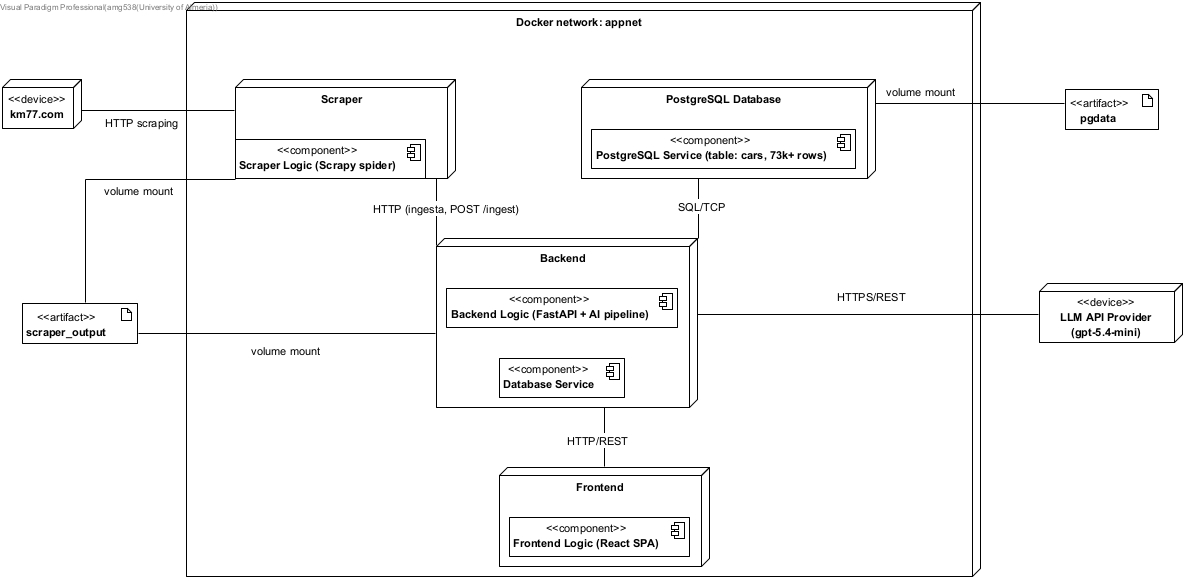
\includegraphics[width=1.1\textwidth]{Figuras/arquitectura.jpg}
    \caption{Diagrama de arquitectura general del sistema.}
    \label{fig:arquitectura}
\end{figure}

El elemento que articula esta arquitectura es la elección de un \textbf{punto de
acceso único a los datos}: el \emph{backend} es el único servicio autorizado a
leer y escribir en la base de datos. El \emph{frontend} nunca consulta la base
de datos directamente, sino que pasa siempre por la API; y el \emph{scraper},
aun produciendo los datos, tampoco los inserta por su cuenta, sino que delega su
ingesta en el \emph{backend} mediante una llamada HTTP. Esta decisión concentra
en un solo lugar la validación, la normalización y el control de acceso, evita
duplicar la lógica de persistencia y garantiza que ningún dato entre en la base
de datos sin haber pasado antes por el mismo proceso de saneamiento.

\subsection*{Comunicación entre servicios}

Los servicios se comunican mediante dos mecanismos complementarios. El principal
es \textbf{HTTP/REST}: la interfaz consume los \emph{endpoints} del \emph{backend}
para listar el catálogo, comparar vehículos y conversar con el asistente, y el
\emph{scraper} invoca el \emph{endpoint} de ingesta cuando termina una
extracción. El secundario es un \textbf{volumen de disco compartido} entre el
\emph{scraper} y el \emph{backend}: el primero escribe en él el archivo con los
datos extraídos y el segundo lo lee durante la ingesta. Este reparto evita que
el \emph{scraper} necesite conocer el esquema de la base de datos o las
credenciales de acceso, y mantiene la frontera entre «producir datos crudos» y
«validar y persistir datos» nítidamente trazada.

Todos los servicios residen en una misma red privada virtual y se descubren
entre sí por su nombre lógico (\texttt{bd}, \texttt{backend}, etc.), sin
necesidad de direcciones fijas. El arranque está ordenado según las dependencias
reales: el \emph{backend} no se inicia hasta que la base de datos responde a su
comprobación de salud, y ni el \emph{frontend} ni el \emph{scraper} arrancan
hasta que el \emph{backend} está operativo. Con ello se elimina toda una clase
de errores transitorios de arranque sin recurrir a esperas arbitrarias. Los
detalles concretos de contenerización y orquestación se describen en el capítulo
de implementación.

\subsection*{Patrón arquitectónico interno del \emph{backend}}

Dentro del \emph{backend}, la organización del código sigue una
\textbf{arquitectura en capas} que separa la exposición HTTP de la lógica de
dominio y del acceso a datos. Se distinguen cuatro niveles:

\begin{itemize}
    \item La capa de \textbf{API} (paquete \texttt{api}) define los
    \emph{endpoints} REST, valida la entrada y traduce las peticiones HTTP en
    llamadas a la lógica de negocio. No contiene reglas de dominio ni SQL.

    \item La capa de \textbf{servicios} (paquete \texttt{services}) concentra la
    lógica de negocio: la normalización de los datos, el acceso a la base de
    datos (a través de un \emph{repositorio}) y la integración con el modelo de
    lenguaje.

    \item La capa de \textbf{modelos} (paquete \texttt{models}) define las
    estructuras de datos con las que trabaja el sistema mediante \emph{Pydantic},
    lo que aporta validación automática y una frontera de tipos explícita.

    \item La capa \textbf{núcleo} (paquete \texttt{core}) reúne la configuración
    transversal y la gestión de la conexión a la base de datos.
\end{itemize}

Esta separación facilita las pruebas (cada capa puede probarse de forma
aislada), localiza los cambios (una modificación en el esquema de la base de
datos afecta al repositorio, no a los \emph{endpoints}) y mantiene las
dependencias dirigidas en un único sentido: la API depende de los servicios y
estos de los modelos y el núcleo, nunca a la inversa.

\section{Modelo de datos}
\label{sec:modelo-datos}

El modelo de datos de \emph{autoAI} gira en torno a un único concepto central:
la \textbf{versión de un vehículo}. El dominio de los automóviles es
naturalmente jerárquico —una \emph{marca} agrupa varios \emph{modelos}, cada
modelo se ofrece en distintos \emph{submodelos} o generaciones, y cada submodelo
incluye varias \emph{versiones} o acabados con motorizaciones y equipamientos
diferentes—, pero es la versión la que constituye la unidad mínima con
significado para el usuario: es a ese nivel donde están definidos el precio, la
potencia, el consumo o las dimensiones concretas. Por ello, la versión es la
entidad sobre la que se construyen las búsquedas, las comparaciones y las
recomendaciones.

Esta entidad se materializa en el sistema a través de dos representaciones
distintas que conviene diferenciar desde el principio, porque reflejan dos
momentos del ciclo de vida del dato:

\begin{itemize}
    \item Una representación \textbf{cruda} (\texttt{CocheScrap}), que recoge los
    datos tal y como se extraen del portal de origen. Todos sus campos son
    cadenas de texto, porque así llegan del \emph{scraping}: incluyen unidades
    («\texttt{177 CV / 130 kW}»), separadores de miles, símbolos de moneda,
    rangos de fechas y marcadores de dato ausente. Esta representación es fiel a
    la fuente, pero inservible para consultar o calcular.

    \item Una representación \textbf{normalizada} (\texttt{Version}), que es el
    modelo canónico del sistema. Cada atributo tiene ya su tipo correcto
    (numérico, fecha, texto), las unidades se han eliminado, los vocabularios se
    han unificado y la ausencia de dato se representa de forma explícita. Es la
    estructura que viaja por toda la aplicación: la que devuelve la base de
    datos, la que consume el pipeline de IA y la que recibe la interfaz.
\end{itemize}

El paso de la primera representación a la segunda es el proceso de normalización,
descrito en la sección~\ref{sec:normalizacion}. Junto a estas dos estructuras
existe una tercera familia de modelos, los \textbf{bloques de respuesta} del
asistente (\texttt{Block}), que no describen vehículos sino el contenido
estructurado que el modelo de lenguaje genera (texto, tablas, gráficas e
imágenes); se detallan en la sección~\ref{sec:diseno-pipeline-ia}.

\subsection{Diseño de la base de datos}
\label{sec:diseno-bd}

La persistencia se resuelve con una base de datos relacional \emph{PostgreSQL}.
La decisión de diseño más característica es que el catálogo se almacena en una
\textbf{única tabla, \texttt{cars}, deliberadamente desnormalizada}, en la que
cada fila representa una versión completa de un vehículo con todos sus atributos.
La jerarquía marca\,$\to$\,modelo\,$\to$\,submodelo\,$\to$\,versión no se modela
con tablas separadas y claves foráneas, sino que se aplana en cuatro columnas de
texto dentro de la misma fila (\texttt{marca}, \texttt{modelo},
\texttt{submodelo}, \texttt{nombre}).

Esta elección, que se aparta de la tercera forma normal que cabría esperar en un
diseño relacional ortodoxo, está justificada por la naturaleza del problema:

\begin{itemize}
    \item \textbf{La carga de trabajo es de solo lectura.} El usuario nunca
    edita el catálogo; este se regenera por completo desde la fuente. No existe,
    por tanto, el riesgo de anomalías de actualización que la normalización
    busca prevenir, que es precisamente su principal motivación.

    \item \textbf{El patrón de acceso dominante es el filtrado multicriterio
    sobre una sola entidad.} Casi todas las consultas (tanto del catálogo como de
    las herramientas de la IA) seleccionan versiones según combinaciones de
    atributos de la propia versión. Una tabla plana resuelve estas consultas sin
    una sola operación de \emph{join}, lo que simplifica drásticamente el
    \emph{repositorio} y mejora el rendimiento.

    \item \textbf{Reduce la complejidad accidental.} Para un catálogo de tamaño
    moderado y que cabe holgadamente en memoria, mantener un esquema en estrella
    o totalmente normalizado añadiría complejidad sin beneficio práctico
    apreciable.
\end{itemize}

\subsubsection*{Estructura de la tabla \texttt{cars}}

La tabla \texttt{cars} reúne veintiséis columnas que se pueden agrupar
conceptualmente en cinco bloques, recogidos en la
tabla~\ref{tab:esquema-cars}. La clave primaria es un identificador entero
autoincremental (\texttt{id}), que es el que el sistema usa internamente para
referirse a cada vehículo —en las comparaciones, en la recuperación de fichas y
en los bloques de imagen generados por la IA—. Además, la columna \texttt{url}
(la dirección de la ficha del vehículo en el portal de origen) está declarada
\texttt{UNIQUE} y desempeña el papel de \textbf{clave de negocio}: identifica de
forma estable una misma versión entre distintas ejecuciones del \emph{scraping},
lo que permite reconocer si un vehículo ya existe y actualizarlo en lugar de
duplicarlo.

\begin{table}[H]
\centering
\begin{tabular}{p{3.2cm}p{9.5cm}}
\hline
\textbf{Bloque} & \textbf{Columnas principales} \\
\hline
Identificación &
\texttt{id} (PK), \texttt{marca}, \texttt{modelo}, \texttt{submodelo},
\texttt{nombre}, \texttt{url} (única), \texttt{foto\_url} \\
\hline
Vigencia &
\texttt{fecha\_inicio}, \texttt{fecha\_fin} (inicio y fin de comercialización) \\
\hline
Precio &
\texttt{precio} (en euros) \\
\hline
Carrocería y \mbox{dimensiones} &
\texttt{carroceria}, \texttt{puertas}, \texttt{plazas}, \texttt{longitud},
\texttt{anchura}, \texttt{altura}, \texttt{capacidad\_maletero} \\
\hline
Mecánica y \mbox{prestaciones} &
\texttt{combustible}, \texttt{potencia}, \texttt{aceleracion},
\texttt{velocidad\_maxima}, \texttt{peso}, \texttt{consumo\_medio},
\texttt{traccion}, \texttt{transmision}, \texttt{numero\_marchas},
\texttt{capacidad\_deposito} \\
\hline
\end{tabular}
\caption{Bloques de atributos de la tabla \texttt{cars}.}
\label{tab:esquema-cars}
\end{table}

Los tipos de cada columna se han elegido para reflejar la semántica del dato y
no su forma de origen. Las magnitudes físicas se almacenan como valores
numéricos con la precisión adecuada (por ejemplo, el precio con dos decimales y
las dimensiones con un decimal en milímetros), las fechas de comercialización
como tipo \texttt{DATE}, los pequeños enteros (puertas, plazas, número de
marchas) como enteros cortos, y los atributos categóricos (combustible,
carrocería, tracción, transmisión) como cadenas que contienen siempre un valor
del vocabulario canónico definido en la normalización.

\subsubsection*{Tratamiento de los datos ausentes}

Una característica esencial del diseño es la admisión explícita de
\textbf{valores nulos} en la mayoría de las columnas de atributos. La fuente de
datos no es uniforme: hay vehículos sin maletero (como los \emph{pick-up}),
motorizaciones híbridas o eléctricas sin un número discreto de marchas, y campos
que el portal sencillamente no registra. Modelar la ausencia con \texttt{NULL}
—en lugar de con valores centinela como un cero o una cadena vacía— es
fundamental porque permite distinguir «este coche pesa cero», que sería un dato
erróneo, de «no se conoce el peso de este coche», que es la situación real. Esta
distinción se propaga a todo el sistema: el \emph{backend} ordena los resultados
colocando siempre los valores nulos al final, y la interfaz los muestra como
«dato no disponible» en lugar de inventar una cifra.

Un caso particular es la \textbf{vigencia}, modelada con el par de fechas
\texttt{fecha\_inicio} y \texttt{fecha\_fin}. La convención es que una
\texttt{fecha\_fin} nula significa que la versión \emph{sigue a la venta hoy};
es decir, el valor nulo no representa aquí un dato desconocido, sino un estado
del mundo (vehículo aún en comercialización). Esta semántica es la que permite
ofrecer al usuario, por defecto, el mercado actual y no versiones
descatalogadas, y es un punto que tanto el \emph{backend} como las instrucciones
del modelo de lenguaje tratan de forma explícita.

\subsubsection*{Índices}

Para sostener el rendimiento de las consultas más frecuentes sin recurrir a
optimizaciones prematuras, el esquema define un conjunto reducido y deliberado de
índices. Se indexan las columnas sobre las que más habitualmente se filtra
(\texttt{marca}, \texttt{modelo}, \texttt{precio}, \texttt{combustible},
\texttt{carroceria}, \texttt{potencia}, \texttt{plazas}) y la columna que
gobierna el orden por defecto del catálogo (\texttt{fecha\_inicio}, ya que las
novedades se muestran primero). Merece mención especial un \textbf{índice
parcial} sobre las versiones vigentes —las que tienen \texttt{fecha\_fin}
nula—: al restringir el índice únicamente a las filas que cumplen esa condición,
se acelera de forma muy eficiente la consulta «solo vehículos a la venta», que es
una de las más recurrentes, ocupando además mucho menos espacio que un índice
completo.

% Diagrama entidad-relación (o, al ser una sola tabla, esquema físico de la
% tabla «cars») mostrando las 26 columnas con sus tipos de datos, la clave
% primaria (id), la restricción UNIQUE sobre url, qué columnas admiten NULL y los
% índices definidos (incluido el índice parcial sobre fecha_fin IS NULL). Sirve
% para visualizar de un vistazo el esquema físico descrito en esta sección.


\begin{figure}[H]
    \centering
	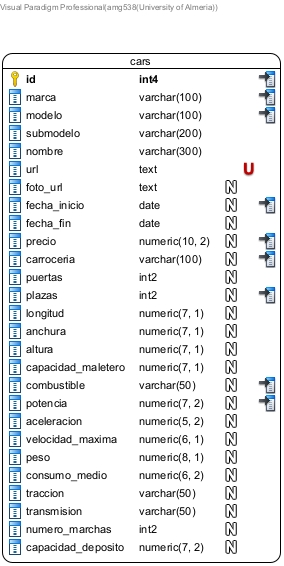
\includegraphics[width=0.4\textwidth]{Figuras/tabla_cars.jpg}
	\caption{Esquema físico de la tabla «cars».}
	\label{fig:tabla-cars}
\end{figure}

\subsection{Normalización de los datos de los vehículos}
\label{sec:normalizacion}

La normalización es, posiblemente, la pieza de diseño más delicada del sistema.
Los datos que llegan del \emph{scraping} son fieles a la fuente pero
heterogéneos y «sucios»: vienen como texto con unidades incrustadas, con
formatos de número propios del español, con rangos de fechas escritos como
cadenas y, sobre todo, con vocabularios inconsistentes y datos implícitos. El
proceso de normalización tiene como misión convertir esa materia prima en el
modelo canónico \texttt{Version}, de forma que el resto del sistema —y en
particular el modelo de lenguaje— pueda razonar sobre datos limpios, tipados y
con un vocabulario cerrado y predecible. Se distinguen tres tareas: el
saneamiento de los valores escalares, la unificación de los vocabularios
categóricos y la persistencia idempotente.

\subsubsection*{Saneamiento de valores escalares}

La parte más mecánica consiste en extraer de cada cadena el valor numérico o la
fecha que contiene, descartando todo lo accesorio. Se aplican reglas
específicas por tipo de campo: de «\texttt{177 CV / 130 kW}» se conserva
únicamente la cifra en caballos; de «\texttt{4.165 mm}» se obtiene el valor en
milímetros eliminando el separador de miles; de «\texttt{7,2 l/100 km}» se extrae
el número cambiando la coma decimal por punto; y los rangos de fechas del tipo
«\texttt{(03/2021 - 09/2023)}» se descomponen en las dos fechas que delimitan la
vigencia. Un principio transversal gobierna todo este proceso: ante un valor
ausente o un marcador de dato faltante (el portal usa un guion), la conversión
\textbf{nunca falla ni inventa}, sino que produce un valor nulo. De este modo,
una sola versión con un campo problemático no aborta la importación del lote
completo.

\subsubsection*{Unificación de vocabularios categóricos}

El reto más interesante del diseño no son los números, sino los atributos
categóricos, y muy especialmente el \textbf{tipo de combustible}. El portal de
origen no clasifica los vehículos por su grado de electrificación: en su campo de
combustible solo indica la fuente del motor de combustión (gasolina, gasóleo o
combinaciones con gas), y deja ese campo vacío para los eléctricos puros. La
información de si un coche es híbrido suave, híbrido autorrecargable o híbrido
enchufable no está en ese campo, sino \emph{implícita} en el nombre comercial de
la versión.

El diseño aborda este problema definiendo un \textbf{vocabulario canónico cerrado
de nueve valores} que codifica, en un único atributo, tanto la fuente fósil como
el nivel de electrificación (tabla~\ref{tab:vocab-combustible}). El proceso de
normalización del combustible determina, por un lado, la base fósil a partir del
campo de origen y, por otro, el nivel de electrificación analizando el texto del
nombre y el submodelo con expresiones regulares que reconocen los distintos
términos comerciales, aplicados en orden de mayor a menor especificidad
(enchufable antes que autorrecargable, y este antes que suave) para evitar
clasificaciones erróneas. Es importante señalar que este vocabulario es el mismo
que después se ofrece al modelo de lenguaje como conjunto cerrado de valores
válidos: unificar aquí el vocabulario es lo que permite que la IA filtre con
precisión más adelante.

\begin{table}[H]
\centering
\begin{tabular}{p{3.5cm}p{9cm}}
\hline
\textbf{Valor canónico} & \textbf{Significado} \\
\hline
\texttt{gasolina}      & Gasolina pura, sin electrificar \\
\texttt{gasoleo}       & Diésel puro, sin electrificar \\
\texttt{gas}           & \emph{Bi-fuel}/flex: gasolina con GLP, gas natural o etanol \\
\texttt{electrico}     & 100\,\% eléctrico (BEV) \\
\texttt{mhev\_gasolina} & Microhíbrido (\emph{mild hybrid} 48\,V) de gasolina \\
\texttt{mhev\_gasoleo}  & Microhíbrido (\emph{mild hybrid} 48\,V) de diésel \\
\texttt{hev\_gasolina}  & Híbrido autorrecargable (\emph{full hybrid}) de gasolina \\
\texttt{phev\_gasolina} & Híbrido enchufable (PHEV) de gasolina \\
\texttt{phev\_gasoleo}  & Híbrido enchufable (PHEV) de diésel \\
\hline
\end{tabular}
\caption{Vocabulario canónico del atributo \texttt{combustible}.}
\label{tab:vocab-combustible}
\end{table}

Un tratamiento análogo, aunque más sencillo, recibe el \textbf{tipo de
carrocería}. El portal emplea sus propias denominaciones (Turismo, SUV/Todoterreno,
Turismo familiar, Monovolumen, Descapotable, Pick Up, etc.), que se traducen a un
vocabulario canónico de nueve categorías (\texttt{berlina}, \texttt{suv},
\texttt{compacto}, \texttt{familiar}, \texttt{coupe}, \texttt{cabrio},
\texttt{monovolumen}, \texttt{pickup}, \texttt{furgoneta}) mediante una
combinación de correspondencias exactas y reglas por subcadena que absorben
además sinónimos habituales (\emph{crossover}, \emph{ranchera}, MPV…). El resto
de atributos categóricos (tracción y transmisión) se canonizan simplemente
pasándolos a minúsculas.

\subsubsection*{Idempotencia}

Una propiedad de diseño exigida a las funciones de normalización de vocabulario
es la \textbf{idempotencia}: aplicar la normalización a un valor ya canónico debe
devolver ese mismo valor sin alterarlo. Esto es importante porque el catálogo se
reimporta periódicamente, y debe poder reprocesarse un dato ya normalizado sin
que se corrompa (por ejemplo, sin que un valor ya en forma canónica se vuelva a
transformar y deje de ser válido). La idempotencia hace que el proceso de
ingesta sea seguro de repetir, lo que simplifica enormemente la operación del
sistema.

\subsubsection*{Persistencia idempotente y tolerante a fallos}

La inserción en la base de datos se ha diseñado también con dos garantías. La
primera es la idempotencia a nivel de fila: la sentencia de inserción utiliza la
cláusula \texttt{ON CONFLICT} sobre la columna \texttt{url} de modo que, si una
versión ya existe (identificada por su clave de negocio), sus datos se
\emph{actualizan} en lugar de provocar un error o un duplicado. Así, el catálogo
converge siempre al estado de la última extracción, tanto si se trata de una
carga inicial como de una actualización.

La segunda garantía es la \textbf{tolerancia a fallos parciales}. Cada versión se
inserta dentro de su propio punto de guardado (\emph{savepoint}) anidado, de
forma que si una fila concreta provoca un error en la base de datos, solo se
revierte esa fila y las demás se conservan. El proceso, además, no se limita a
guardar: devuelve un informe detallado del resultado de la importación —cuántos
registros se leyeron, cuántos se validaron correctamente, cuántos se normalizaron
y cuántos se persistieron, junto con la lista de los que fallaron y por qué—.
Este enfoque prioriza la \emph{robustez} sobre la atomicidad estricta: dado que
los datos provienen de un \emph{scraping} de una web externa y, por su
naturaleza, son imperfectos, es preferible cargar todo lo que sea correcto e
informar de lo que no, antes que rechazar un lote completo por unas pocas filas
defectuosas.

% Diagrama de flujo del proceso de normalización e ingesta. Debe mostrar
% la cadena: archivo JSON del scraper -> validación a CocheScrap (texto crudo) ->
% normalización a Version (tipos correctos, vocabularios canónicos, NULLs) ->
% inserción con ON CONFLICT/savepoint por fila -> informe de resultados (leídos,
% validados, normalizados, guardados, errores). Conviene resaltar los puntos
% donde un fallo individual se aísla sin abortar el lote.

\begin{figure}[H]
    \centering
	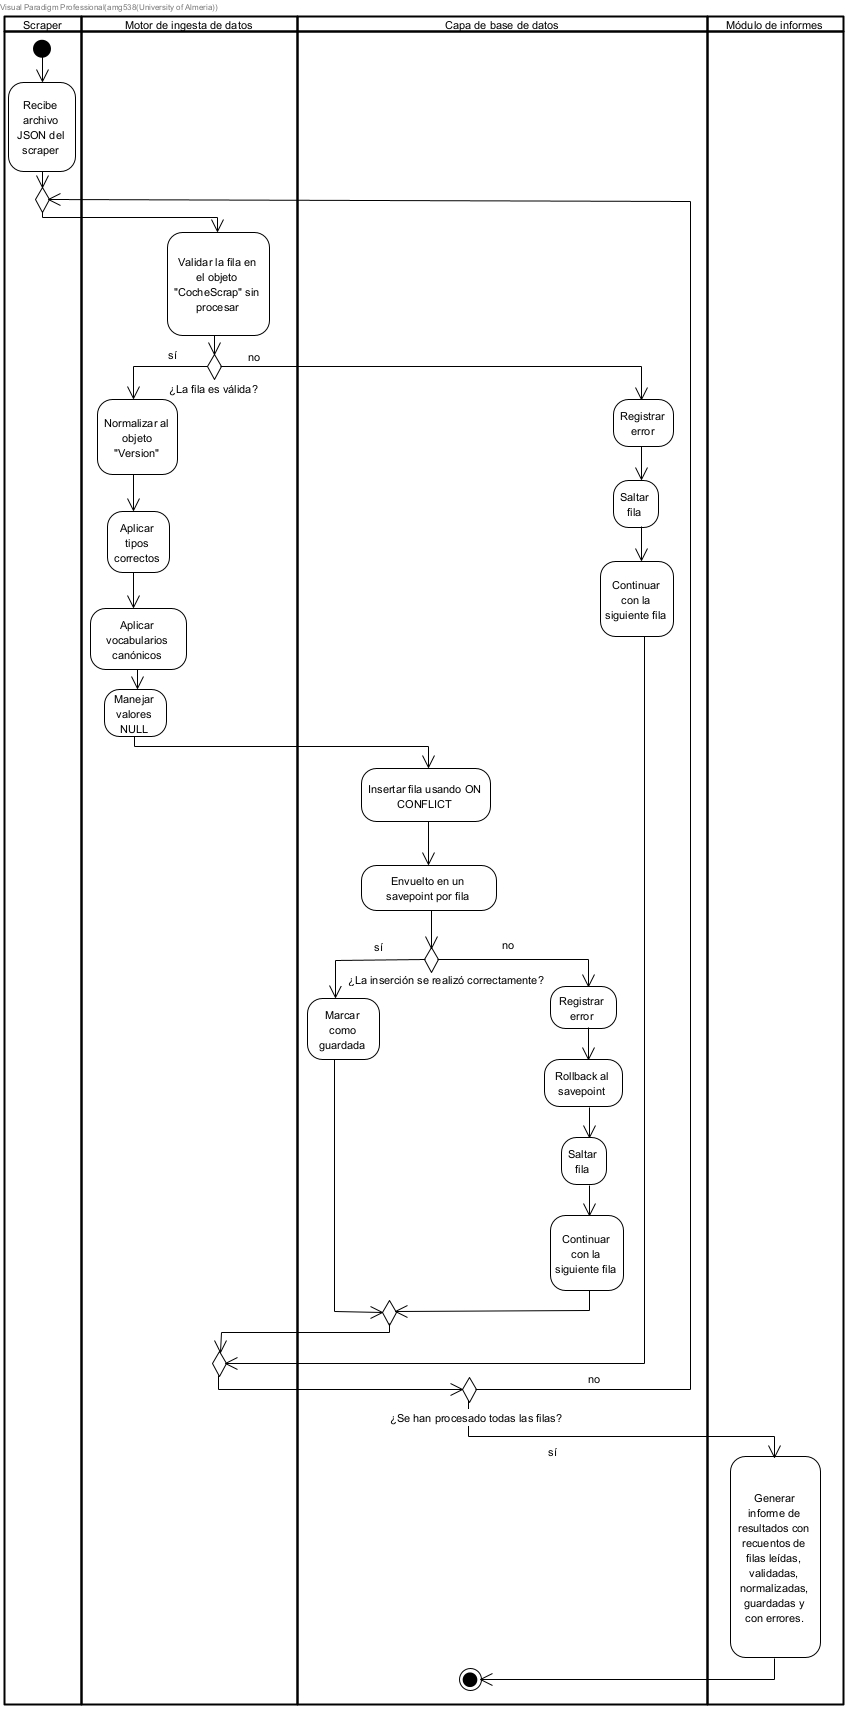
\includegraphics[width=0.7\textwidth]{Figuras/normalizacion.jpg}
	\caption{Diagrama de flujo del proceso de normalización e ingesta.}
	\label{fig:normalizacion}
\end{figure}

\section{Diseño del \emph{backend} (API REST)}
\label{sec:diseno-backend}

El \emph{backend} es el núcleo lógico del sistema y expone sus capacidades a
través de una \textbf{API REST}. Su diseño persigue tres metas: ofrecer a la
interfaz un contrato de datos claro y tipado, mantener la lógica de acceso a la
base de datos centralizada y segura, y servir de orquestador para el pipeline de
inteligencia artificial. La API se organiza en torno a dos grandes familias de
\emph{endpoints} —los del catálogo y comparador, de naturaleza determinista, y
el del asistente conversacional, de naturaleza generativa—, más un par de
\emph{endpoints} de servicio. La tabla~\ref{tab:endpoints} resume el conjunto.

\begin{table}[H]
\centering
\begin{tabular}{p{2.0cm}p{4.3cm}p{6.0cm}}
\hline
\textbf{Método} & \textbf{Ruta} & \textbf{Función} \\
\hline
GET  & \texttt{/api/cars} & Lista de versiones filtrada y paginada (catálogo) \\
GET  & \texttt{/api/cars/\{id\}} & Ficha completa de una versión \\
POST & \texttt{/api/compare} & Fichas de varias versiones para comparar \\
GET  & \texttt{/api/filters/meta} & Valores distintos disponibles para los filtros \\
POST & \texttt{/chat} & Consulta en lenguaje natural al asistente \\
POST & \texttt{/ingest} & Ingesta de un archivo del \emph{scraper} (interno) \\
GET  & \texttt{/health} & Comprobación de estado del servicio \\
\hline
\end{tabular}
\caption{\emph{Endpoints} de la API REST del \emph{backend}.}
\label{tab:endpoints}
\end{table}

\subsubsection*{Endpoints del catálogo y comparador}

Los \emph{endpoints} del catálogo dan servicio a la navegación clásica de la
interfaz. El de listado acepta como parámetros de consulta un conjunto de
filtros (marca, modelo, combustible, carrocería, tracción, transmisión y rangos
de precio, potencia y plazas) junto con la paginación, y devuelve la lista de
versiones que los cumplen. El de ficha individual recupera un vehículo por su
identificador, y el de comparación recibe una lista de identificadores y devuelve
sus fichas completas. Un \emph{endpoint} auxiliar, el de metadatos de filtros,
devuelve los valores realmente presentes en la base de datos para cada atributo
categórico, lo que permite a la interfaz poblar dinámicamente sus desplegables
sin codificar los valores manualmente.

Una decisión de diseño relevante es que las respuestas de estos \emph{endpoints}
se ajustan exactamente al modelo canónico \texttt{Version}. El esquema de la
respuesta se declara de forma explícita, lo que aporta tres beneficios: la
documentación interactiva de la API se genera automáticamente, la validación de
la salida está garantizada por el \emph{framework}, y la interfaz puede definir
un tipo «espejo» que refleja exactamente esa estructura, de modo que el contrato
de datos entre \emph{frontend} y \emph{backend} queda fijado y verificable en
ambos extremos.

\subsubsection*{El repositorio y la construcción segura de consultas}

Toda la interacción con la base de datos se concentra en un único módulo, el
\textbf{repositorio de vehículos}, que actúa como frontera entre la lógica de
negocio y el SQL. Este patrón evita que las sentencias SQL se dispersen por el
código y permite construir las consultas de forma dinámica a partir de un
diccionario de filtros: el repositorio traduce cada filtro presente en una
condición de la cláusula \texttt{WHERE} y omite los ausentes, soportando tanto
igualdades simples como filtros de pertenencia a un conjunto (por ejemplo, varios
tipos de combustible a la vez) y rangos numéricos.

El aspecto más importante de este módulo es su \textbf{tratamiento de la
seguridad}. Todos los valores aportados por el usuario se pasan a la consulta
como \textbf{parámetros vinculados}, nunca por interpolación de cadenas, lo que
elimina por construcción el riesgo de inyección de SQL. En los pocos casos en que
es inevitable insertar un identificador en la propia estructura de la consulta
—por ejemplo, el nombre de la columna por la que ordenar o agregar—, ese
identificador se valida previamente contra una \textbf{lista blanca} de valores
permitidos: el nombre de ordenación se busca en un diccionario cerrado de
órdenes válidos, y los campos y operaciones de agregación se comprueban contra
conjuntos predefinidos. Cualquier valor fuera de esas listas se rechaza antes de
construir la consulta. De este modo se concilian la flexibilidad de las consultas
dinámicas con la imposibilidad de que un valor arbitrario llegue al motor de la
base de datos.

\subsubsection*{Endpoints de servicio y configuración}

Completan la API dos \emph{endpoints} de servicio. El de comprobación de estado
permite que la orquestación verifique que el \emph{backend} está vivo antes de
arrancar los servicios que dependen de él. El de ingesta es el que invoca el
\emph{scraper} para solicitar la carga de un archivo; por seguridad, su diseño
restringe el acceso al directorio compartido y rechaza cualquier intento de
acceder a rutas fuera de él. Toda la configuración sensible del \emph{backend}
(la cadena de conexión a la base de datos, la clave del proveedor de IA, los
orígenes permitidos para las peticiones de la interfaz) se externaliza mediante
variables de entorno y se valida al arranque, de forma que el código no contiene
ningún secreto y el comportamiento puede ajustarse entre entornos sin
recompilar. Adicionalmente, el \emph{backend} incorpora sendos mecanismos
opcionales de limitación de frecuencia de peticiones y de autenticación por
clave para los \emph{endpoints} sensibles, desactivados por defecto y activables
por configuración.

\section{Diseño del pipeline de consulta con IA}
\label{sec:diseno-pipeline-ia}

El pipeline de inteligencia artificial es el componente diferencial de
\emph{autoAI} y el que materializa su objetivo principal: permitir que un usuario
exprese sus necesidades en \textbf{lenguaje natural} y reciba una recomendación
\textbf{fundamentada en datos reales}. El reto de diseño central es conciliar dos
mundos en tensión: la flexibilidad y la fluidez de un modelo de lenguaje, que
puede interpretar peticiones ambiguas y redactar respuestas naturales, con el
\textbf{rigor factual} de una base de datos, que es la única fuente legítima de
cifras. La estrategia adoptada para resolver esta tensión es no permitir nunca
que el modelo invente datos, sino obligarlo a obtenerlos de la base de datos a
través de un conjunto acotado de herramientas, en un patrón conocido como
\emph{tool-calling}.

\subsubsection*{De lenguaje natural a filtros estructurados: las herramientas}

En lugar de pedir al modelo que genere SQL —lo que sería potente pero
arriesgado—, el diseño le ofrece un \textbf{catálogo cerrado de cuatro
herramientas} de alto nivel que encapsulan las operaciones que el sistema sabe
hacer con seguridad (tabla~\ref{tab:tools}). La tarea del modelo se reduce
entonces a traducir la intención del usuario en una llamada a la herramienta
adecuada con los argumentos correctos; es decir, a convertir el lenguaje natural
en un conjunto de \textbf{filtros estructurados}.

\begin{table}[H]
\centering
\begin{tabular}{p{3.0cm}p{9.5cm}}
\hline
\textbf{Herramienta} & \textbf{Función} \\
\hline
\texttt{buscar\_coches} &
Busca versiones que cumplen unos filtros, con orden y límite opcionales \\
\texttt{obtener\_coche} &
Devuelve la ficha completa de un vehículo por su identificador \\
\texttt{comparar} &
Devuelve las fichas de varios vehículos para compararlos \\
\texttt{agregar} &
Calcula una agregación (recuento, media, mínimo, máximo) sobre un campo,
opcionalmente agrupada; es la fuente de las gráficas \\
\hline
\end{tabular}
\caption{Herramientas (\emph{tools}) disponibles para el modelo de lenguaje.}
\label{tab:tools}
\end{table}

La clave del diseño está en la \textbf{especificación de los argumentos} de
estas herramientas. El esquema de filtros que se entrega al modelo no es una
lista libre, sino un contrato estricto: enumera explícitamente los atributos por
los que se puede filtrar y, para los categóricos, restringe los valores
admisibles al vocabulario canónico definido en la normalización. Es aquí donde la
inversión hecha en la unificación de vocabularios rinde sus frutos: como el campo
de combustible solo admite los nueve valores canónicos, el modelo no puede pedir
un «híbrido» genérico ni un «diésel» con otra grafía, sino que debe traducir la
intención del usuario a los valores exactos que existen en la base de datos. El
propio esquema incluye, a modo de instrucciones, las equivalencias entre el
lenguaje coloquial y el vocabulario canónico, lo que guía al modelo en esa
traducción.

\subsubsection*{El bucle de \emph{tool-calling} sobre datos reales}

El corazón del pipeline es un \textbf{bucle de razonamiento} que alterna entre el
modelo de lenguaje y la ejecución de herramientas. Su funcionamiento es el
siguiente: se envía al modelo la conversación junto con la descripción de las
herramientas; si el modelo decide llamar a una o varias, el \emph{backend} las
ejecuta realmente contra la base de datos y le devuelve los resultados; el modelo
puede entonces razonar sobre esos datos y decidir si necesita más información
(refinar la búsqueda, comparar, agregar) o si ya está en condiciones de
responder. El ciclo se repite hasta que el modelo deja de pedir herramientas, con
un \textbf{límite máximo de iteraciones} que actúa como salvaguarda para evitar
bucles infinitos y acotar el coste de cada consulta.

Este diseño garantiza la invariante fundamental del sistema: \textbf{toda cifra
que aparece en una respuesta procede de una consulta real a la base de datos}.
El modelo aporta la interpretación, la estrategia de búsqueda y la redacción,
pero los datos los pone siempre la base de datos. Sobre esta invariante se
articula además un comportamiento experto, codificado en las instrucciones de
sistema que acompañan a cada consulta: el modelo recibe directrices sobre cómo
interpretar peticiones vagas («algo para la familia», «un coche para ciudad»)
traduciéndolas a filtros concretos, cómo priorizar por defecto el mercado actual,
cómo actuar cuando el usuario filtra por un atributo que el sistema no soporta
(explicarlo y ofrecer igualmente una búsqueda aproximada) y cómo tratar casos
delicados como las unidades de consumo de los híbridos enchufables.

Un matiz de diseño interesante distingue entre \textbf{consultas objetivas y
consultas exploratorias}. Cuando el usuario pide algo con un criterio inequívoco
(«el más barato», «el más potente»), la búsqueda devuelve exactamente ese
resultado de forma determinista. Pero cuando la petición es cualitativa y sin un
orden objetivo («un coche bonito para ciudad»), el sistema recupera un conjunto
de candidatos más amplio y selecciona entre ellos con un muestreo sesgado hacia
los más relevantes, de manera que dos consultas parecidas no devuelvan siempre
exactamente los mismos vehículos. Con ello se evita que el asistente resulte
repetitivo sin que por ello se muestren opciones de peor calidad.

\subsubsection*{Generación de respuestas estructuradas y explicadas}

Una recomendación de coches no se expresa bien solo con texto: a menudo requiere
una tabla comparativa, una gráfica de precios o la fotografía del vehículo. Por
eso, la respuesta del asistente no es una cadena de texto plano, sino un
documento estructurado compuesto por una secuencia de \textbf{bloques
tipados}. Se definen cuatro tipos de bloque: texto (en formato \emph{Markdown}),
tabla, gráfica (de barras o radar) e imagen. El modelo, una vez ha reunido los
datos a través de las herramientas, emite una respuesta final que se ajusta de
forma estricta a este esquema de bloques, lo que permite a la interfaz
renderizar cada uno con el componente adecuado.

Este enfoque exige una \textbf{segunda fase} en el pipeline, separada del bucle
de herramientas: una vez recopilados todos los datos, se realiza una última
llamada al modelo solicitándole que produzca el documento de bloques en un
formato verificable. El \emph{backend} valida que la respuesta cumple el esquema
y, si no lo cumple, reintenta una vez indicándole el error; si tampoco así se
obtiene una respuesta válida, se entrega un bloque de texto de reserva en lugar
de propagar un fallo a la interfaz.

Dos decisiones de diseño refuerzan en esta fase la integridad de los datos. La
primera afecta a las \textbf{imágenes}: para evitar que el modelo invente o
altere direcciones de fotografías, se le prohíbe emitir URLs; en su lugar, un
bloque de imagen solo contiene el identificador del vehículo, y es el
\emph{backend} quien, en un paso posterior de «hidratación», recupera de la base
de datos la URL real de la foto y la inserta en el bloque (descartándolo si el
vehículo no existe o no tiene imagen). La segunda afecta a las
\textbf{gráficas}: estas se alimentan exclusivamente de la salida de la
herramienta de agregación, de modo que las barras de un gráfico reflejan siempre
valores calculados por la base de datos y no estimaciones del modelo; las
etiquetas, unidades y títulos son metadatos de presentación que nunca modifican
las cifras subyacentes. En conjunto, estas medidas trasladan la invariante de
«no inventar datos» también a los elementos visuales de la respuesta.

% Diagrama de secuencia del pipeline de IA. Debe representar el flujo
% completo de una consulta: usuario -> frontend -> backend (/chat) -> [bucle:
% backend <-> modelo de lenguaje pidiendo herramientas, y backend <-> base de
% datos ejecutándolas] -> segunda llamada al modelo para el documento de bloques
% -> validación del esquema (con el reintento) -> hidratación de imágenes desde
% la base de datos -> respuesta de bloques al frontend. Conviene marcar las dos
% fases (bucle de tool-calling y generación del envelope) y el límite de
% iteraciones.

\begin{figure}[H]
    \centering
	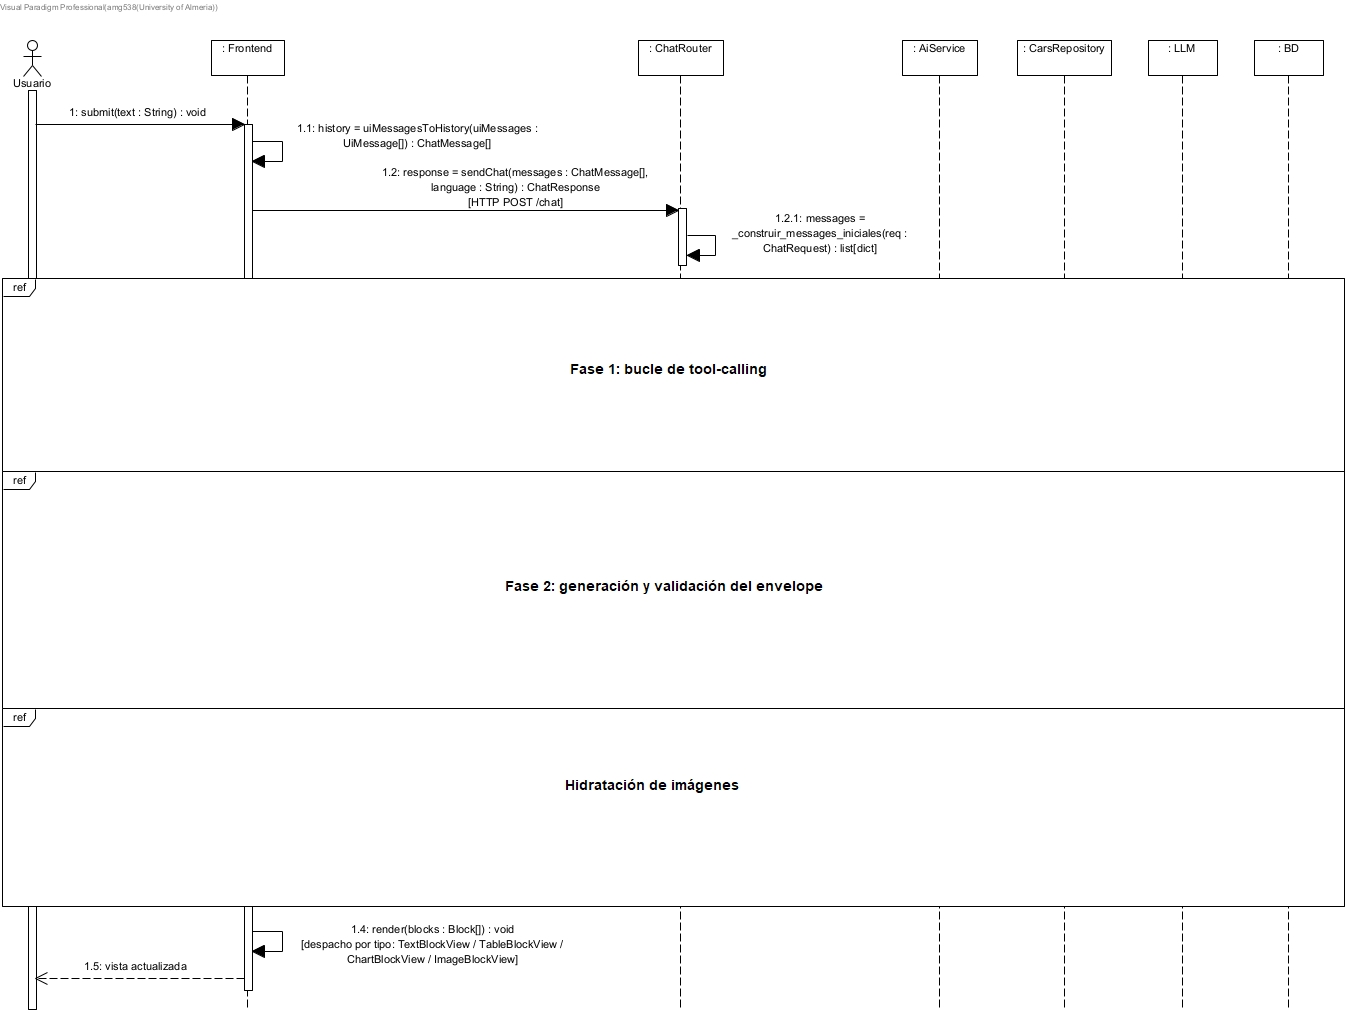
\includegraphics[width=1\textwidth]{Figuras/consulta_general.jpg}
	\caption{Diagrama de secuencia del pipeline de IA. Vista general.}
	\label{fig:consulta-general}
\end{figure}

\begin{figure}[H]
    \centering
	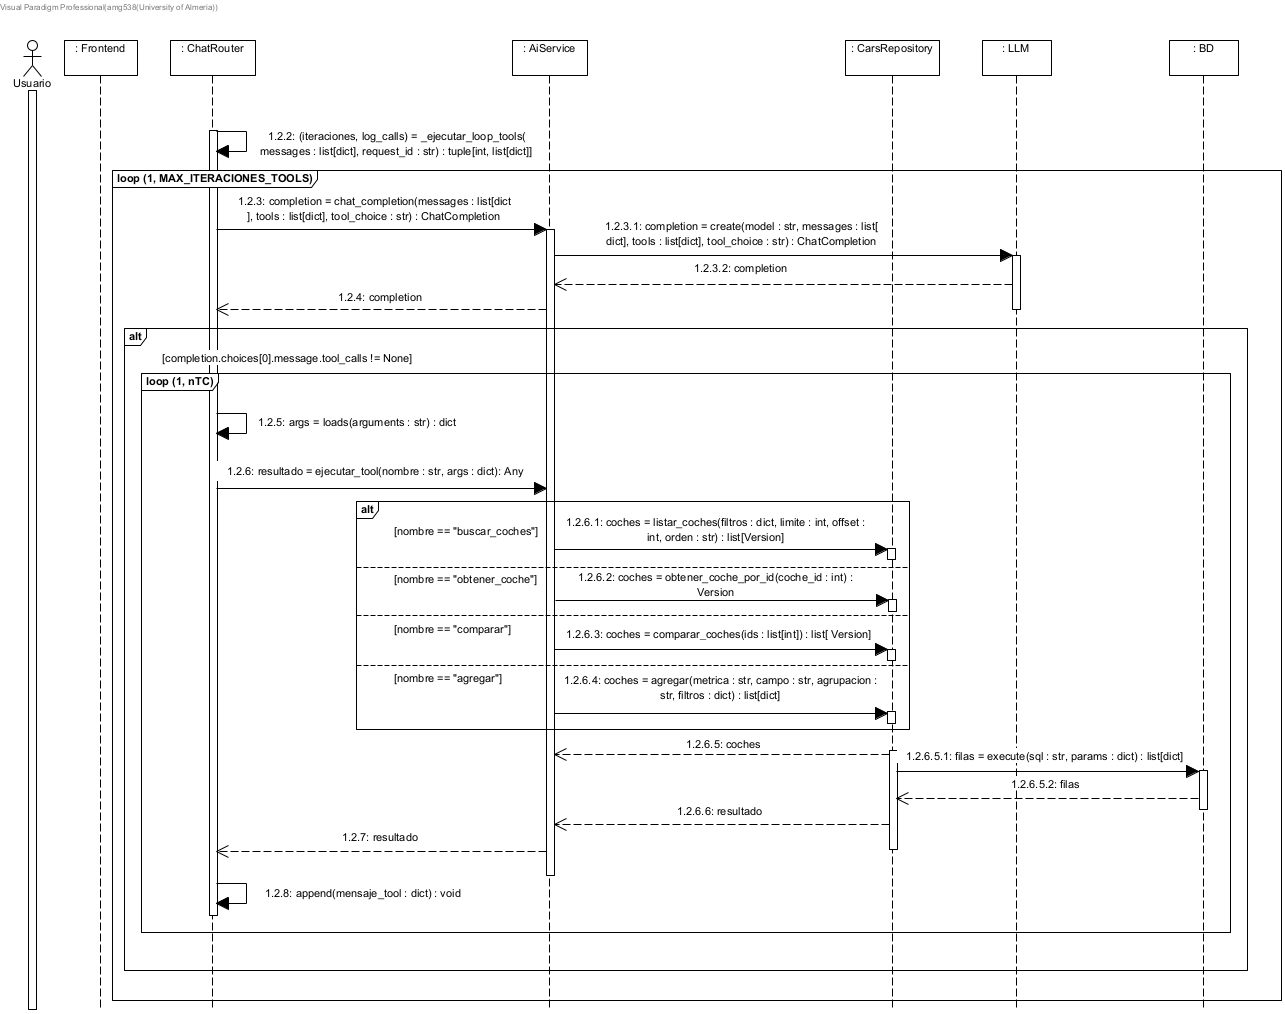
\includegraphics[width=1\textwidth]{Figuras/consulta_fase1.jpg}
	\caption{Diagrama de secuencia del pipeline de IA. Bucle de tool-calling.}
	\label{fig:consulta-fase1}
\end{figure}

\begin{figure}[H]
    \centering
	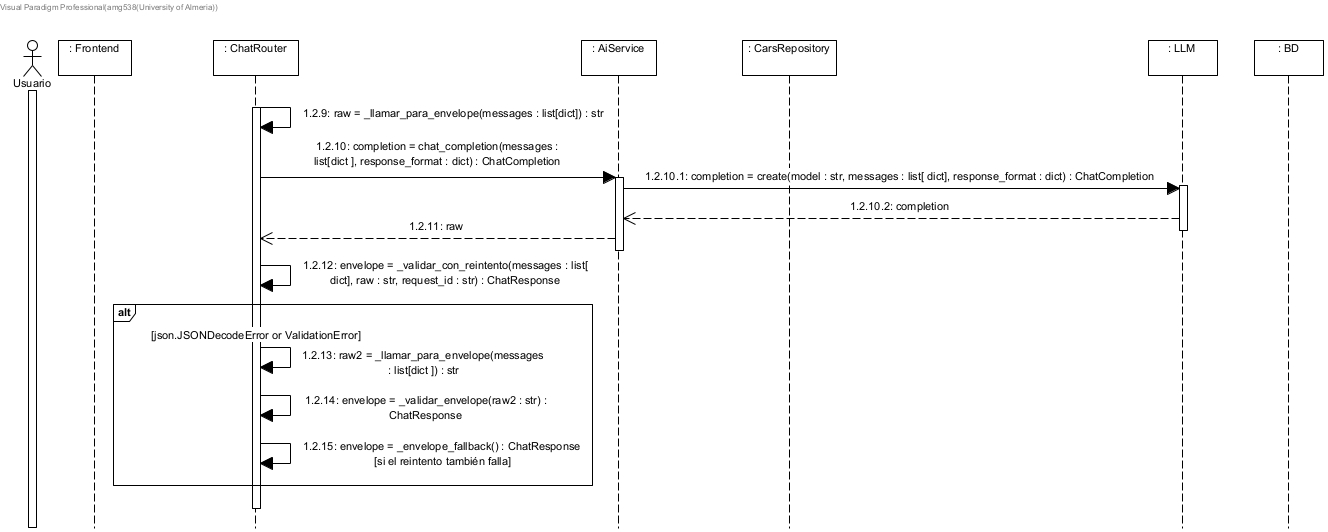
\includegraphics[width=1\textwidth]{Figuras/consulta_fase2.jpg}
	\caption{Diagrama de secuencia del pipeline de IA. Generación del envelope.}
	\label{fig:consulta-fase2}
\end{figure}

\begin{figure}[H]
    \centering
	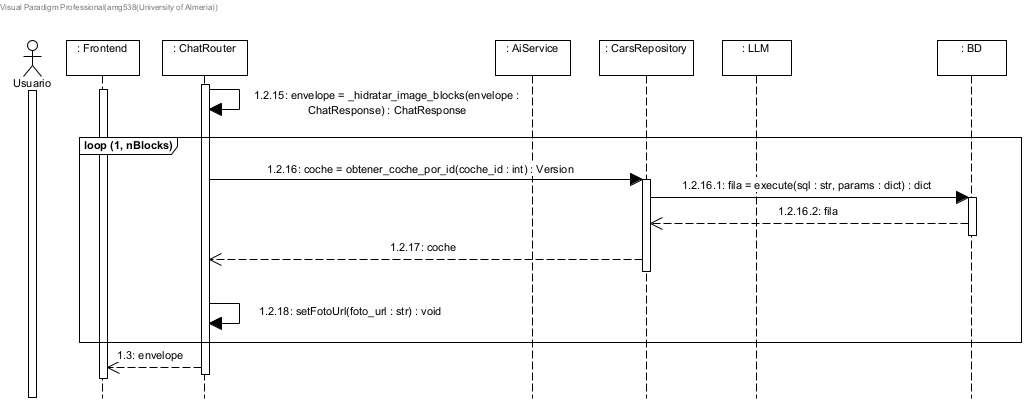
\includegraphics[width=1\textwidth]{Figuras/consulta_hidratacion.jpg}
	\caption{Diagrama de secuencia del pipeline de IA. Hidratación de imágenes.}
	\label{fig:consulta-hidratacion}
\end{figure}

\section{Diseño de la interfaz de usuario}
\label{sec:diseno-interfaz}

La interfaz de usuario se ha diseñado como una \textbf{aplicación web de página
única} que ofrece una experiencia fluida y sin recargas, organizada en torno a
una barra lateral de navegación que da acceso a sus cuatro áreas funcionales: el
\textbf{asistente conversacional}, el \textbf{catálogo}, el \textbf{historial} de
conversaciones y los \textbf{favoritos}. El criterio rector del diseño es
ofrecer dos modos de exploración complementarios sobre el mismo catálogo: uno
\emph{conversacional}, guiado por la IA, para el usuario que prefiere expresar
sus necesidades con sus propias palabras; y otro \emph{estructurado}, mediante
filtros explícitos, para quien prefiere acotar la búsqueda por su cuenta.

\subsubsection*{Interfaz conversacional}

El asistente es la vista principal y se presenta inicialmente con una pantalla de
bienvenida que invita a escribir la primera consulta. A partir de ahí, la
interacción adopta la forma familiar de una conversación, en la que se alternan
los mensajes del usuario y las respuestas del asistente. El reto de diseño
específico de esta vista es la \textbf{renderización de las respuestas
estructuradas}: como la respuesta del \emph{backend} es una secuencia de bloques
tipados, la interfaz recorre esos bloques y delega cada uno en un componente
especializado —el texto se interpreta como \emph{Markdown}, las tablas se pintan
como tablas con desplazamiento horizontal, las gráficas se dibujan con una
biblioteca de visualización y las imágenes se muestran como fichas con una acción
para añadir el vehículo a favoritos—. Este mecanismo de despacho por tipo de
bloque es el que permite que una misma respuesta combine, por ejemplo, un párrafo
introductorio, una tabla comparativa y una gráfica de precios.

El diseño cuida varios detalles de la experiencia conversacional: mientras el
\emph{backend} procesa la consulta se muestra un indicador de escritura, la vista
se desplaza automáticamente al último mensaje, los errores de comunicación se
presentan como un mensaje del asistente en lugar de como un fallo abrupto, y
junto al campo de entrada figura de forma permanente un aviso de que la IA puede
cometer errores, en línea con un uso responsable de la herramienta.

% Captura de pantalla de la interfaz conversacional, idealmente con una
% respuesta del asistente que combine varios tipos de bloque (texto introductorio,
% una tabla comparativa y una gráfica de barras) para ilustrar el renderizado de
% respuestas estructuradas.

\begin{figure}[H]
    \centering
	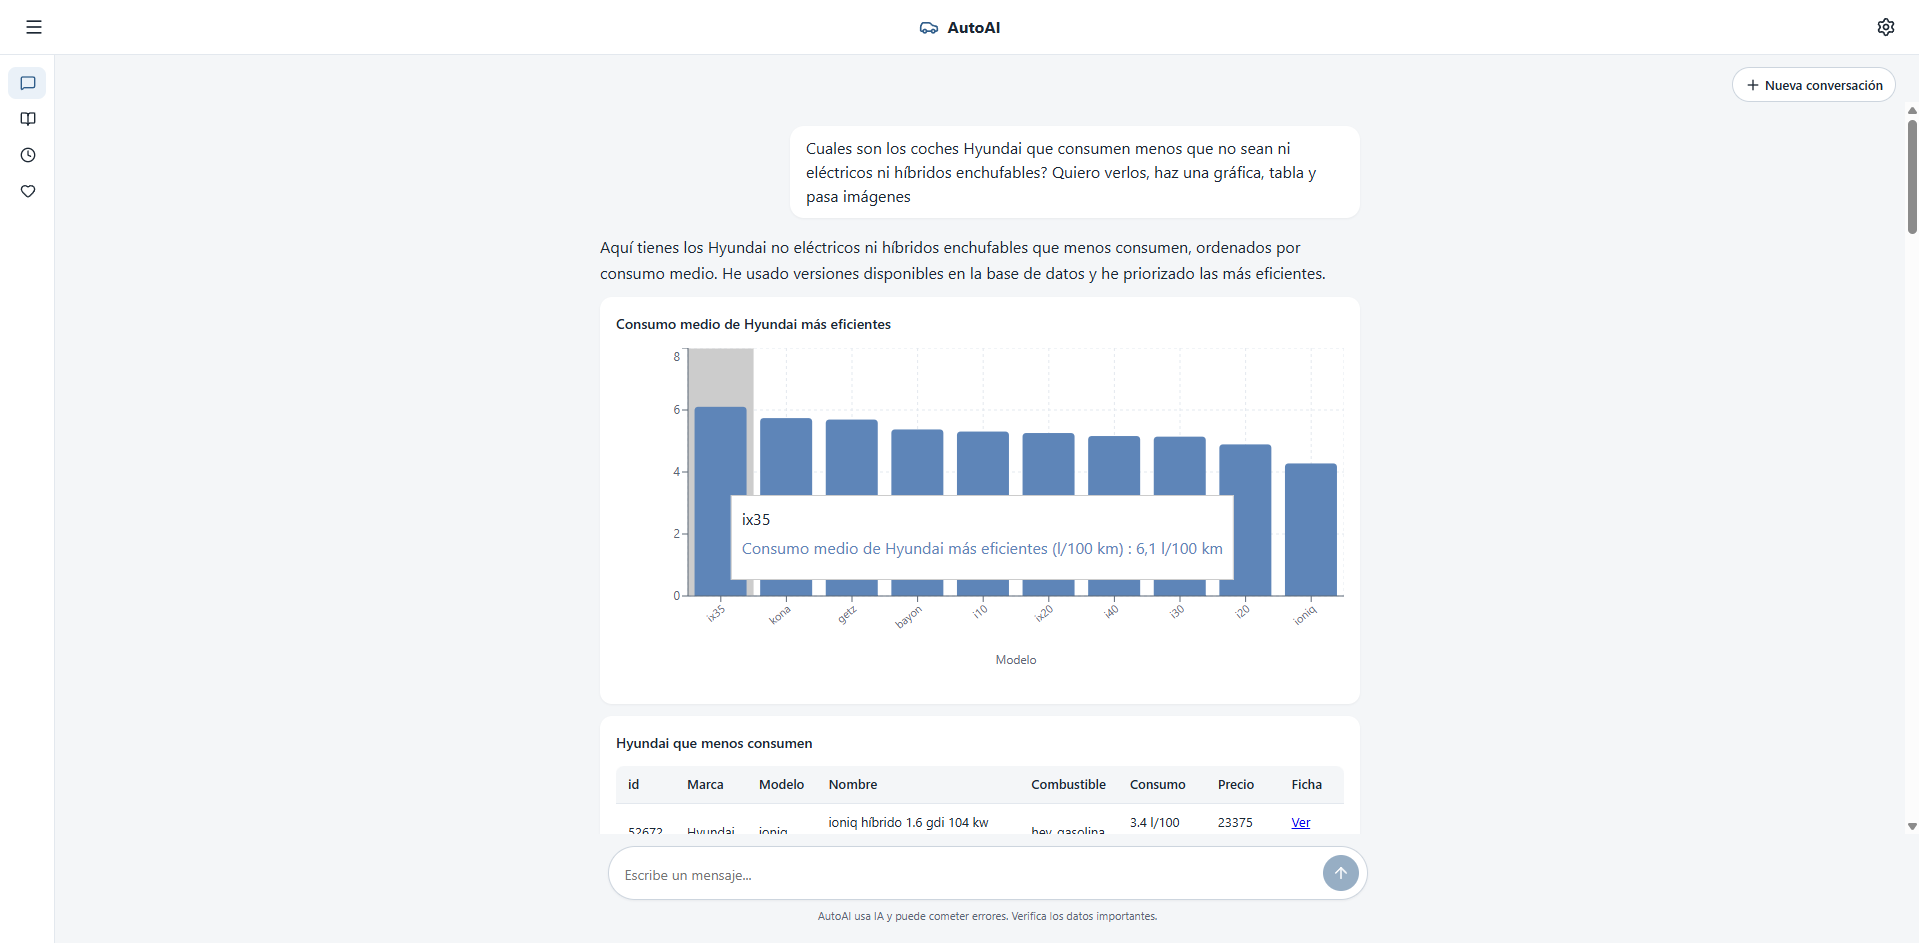
\includegraphics[width=1\textwidth]{Figuras/conversacion_grafica.png}
	\caption{Interfaz conversacional con respuesta de gráfica.}
	\label{fig:conversacion-grafica}
\end{figure}

\begin{figure}[H]
    \centering
	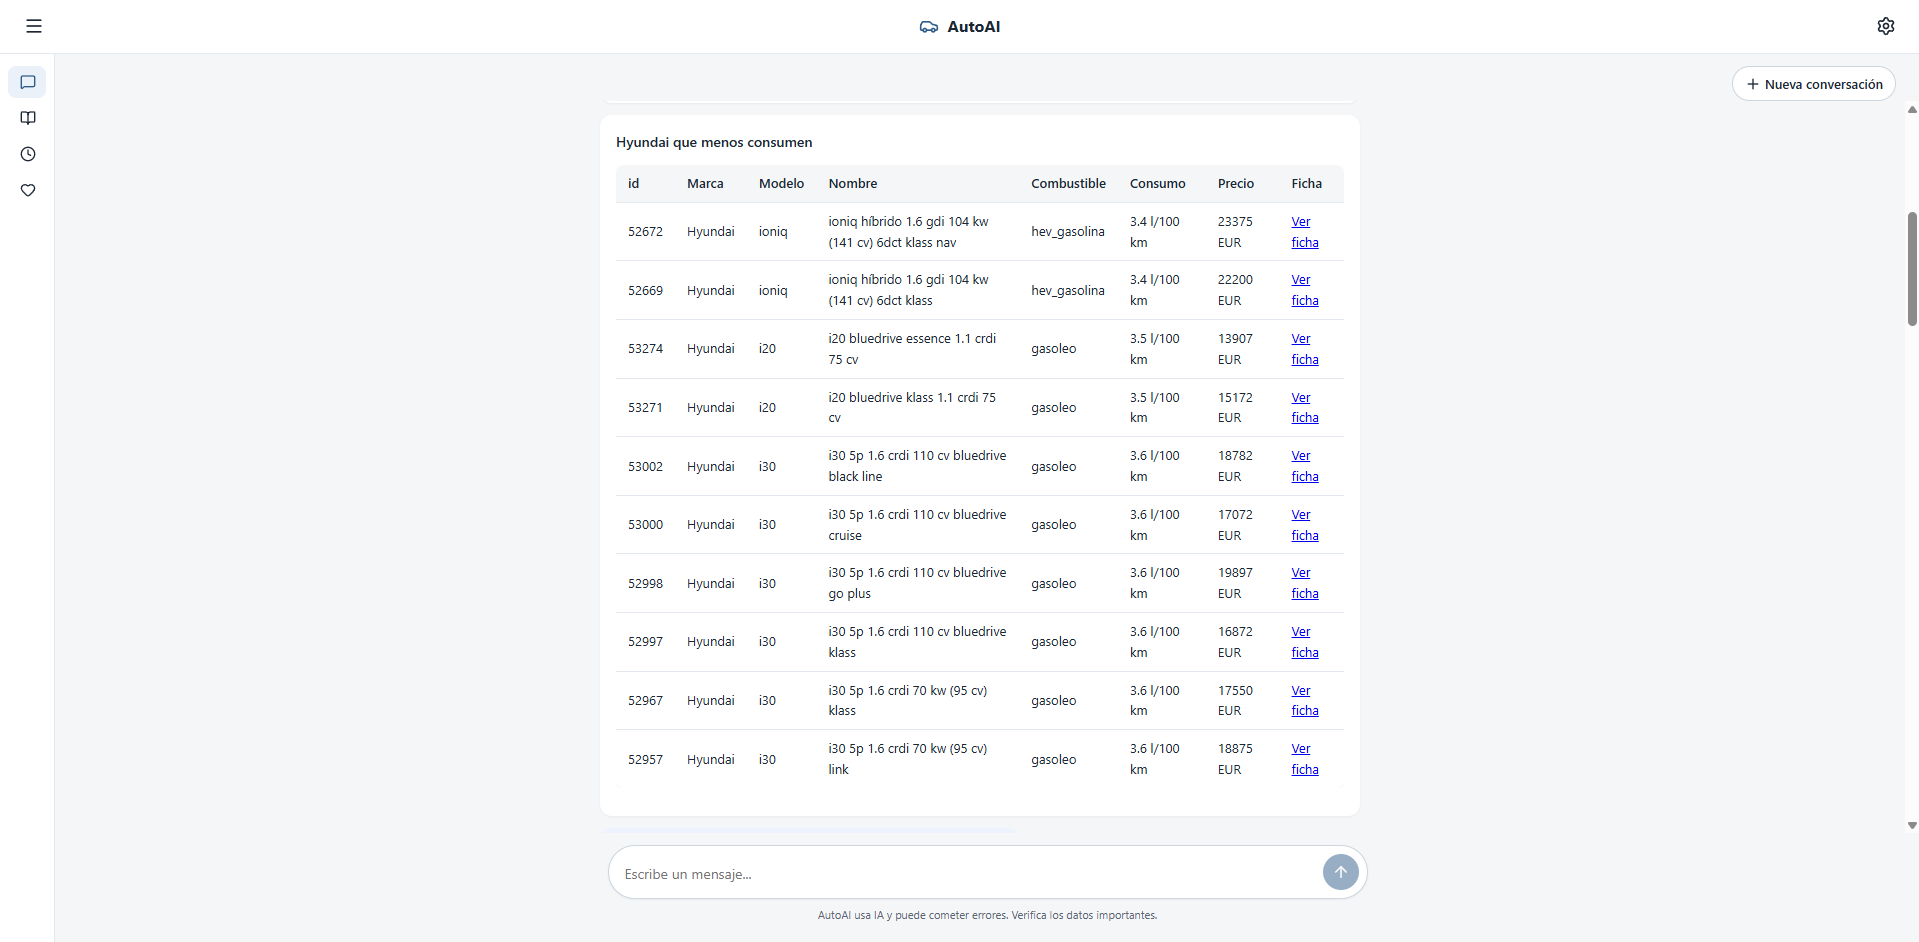
\includegraphics[width=1\textwidth]{Figuras/conversacion_tabla.png}
	\caption{Interfaz conversacional con respuesta de tabla.}
	\label{fig:conversacion-tabla}
\end{figure}

\begin{figure}[H]
    \centering
	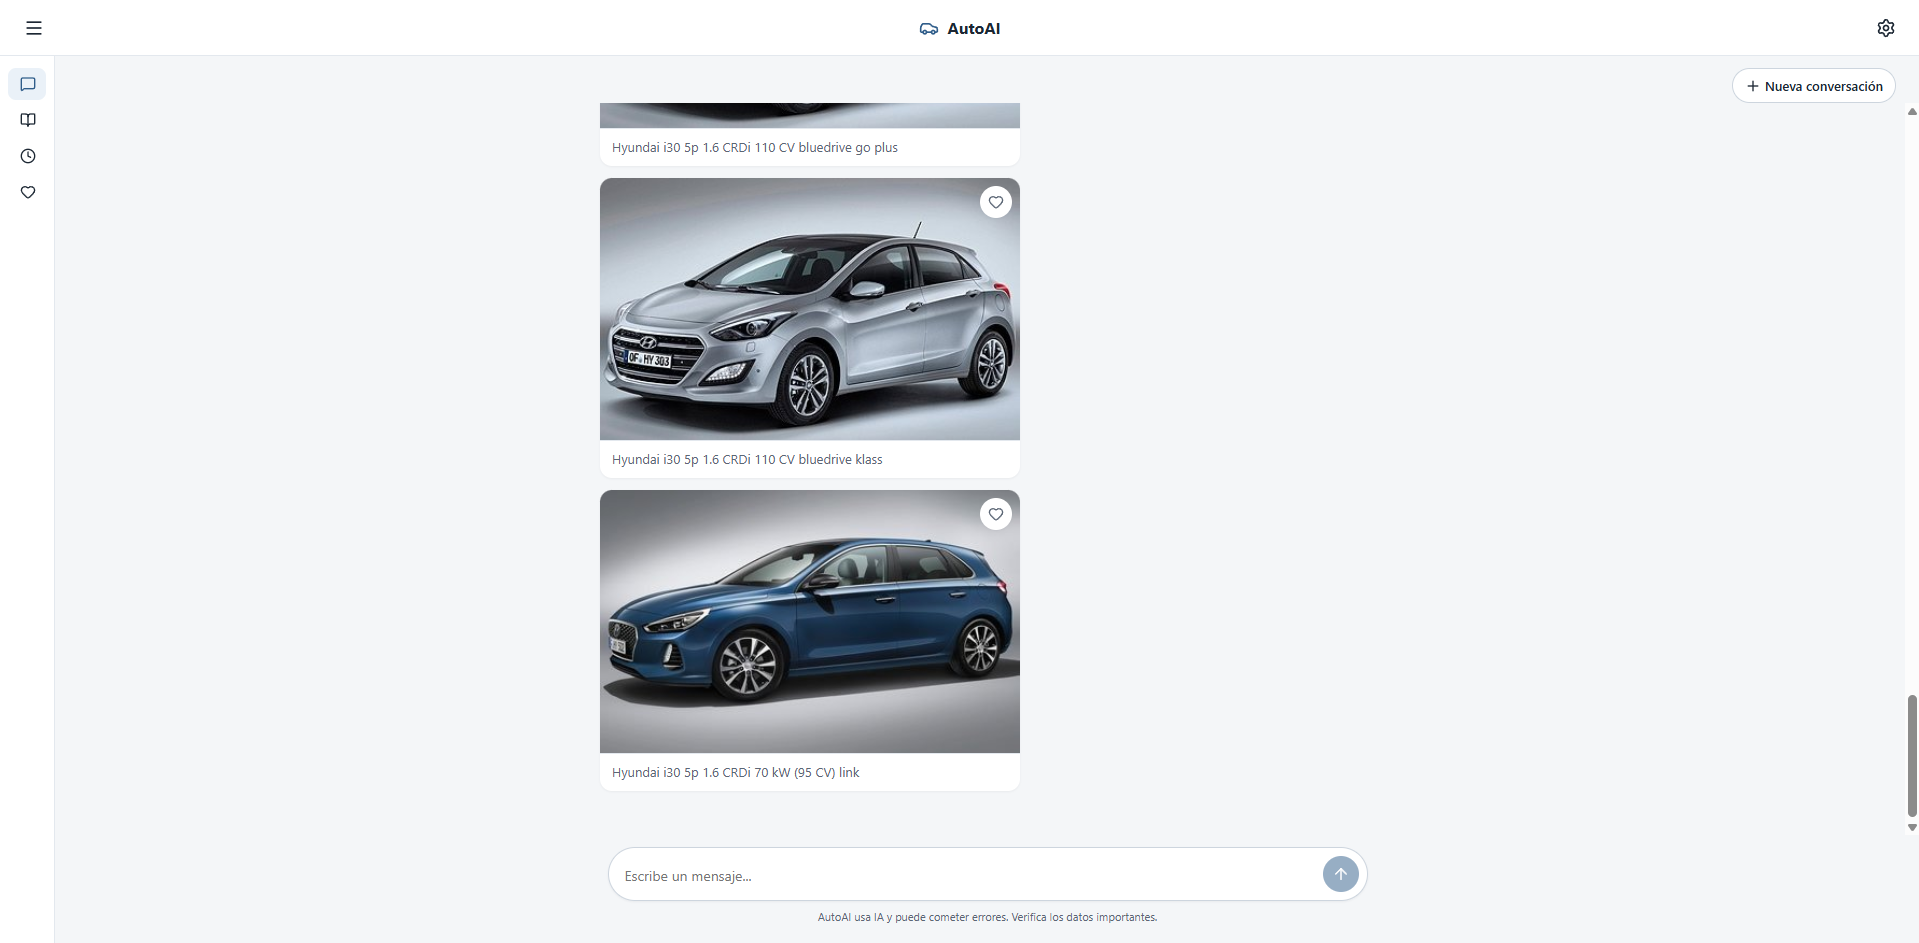
\includegraphics[width=1\textwidth]{Figuras/conversacion_imagenes.png}
	\caption{Interfaz conversacional con respuesta de imágenes.}
	\label{fig:conversacion-imagenes}
\end{figure}

\subsubsection*{Catálogo, filtros y comparador}

El catálogo ofrece la vía de exploración estructurada. Presenta los vehículos en
una rejilla de tarjetas y, sobre ella, un panel de filtros que se construye
dinámicamente a partir de los metadatos que expone el \emph{backend}: los
desplegables de marca, combustible, carrocería, tracción y transmisión se pueblan
con los valores realmente presentes en la base de datos, lo que evita ofrecer
opciones sin resultados. Se complementan con campos para acotar rangos de precio,
potencia y número de plazas, y con un buscador de modelo por texto. Los
resultados se entregan paginados, y la vista contempla de forma explícita los
estados de carga (mostrando una rejilla de marcadores de posición), de error (con
opción de reintento) y de búsqueda sin resultados, de modo que la interfaz nunca
queda en un estado ambiguo.

% Captura de pantalla de la vista de catálogo, mostrando el panel de
% filtros (desplegables de marca/combustible/carrocería/tracción/transmisión y
% campos de rango de precio/potencia/plazas) y la rejilla de tarjetas de
% vehículos con su paginación.

\begin{figure}[H]
    \centering
	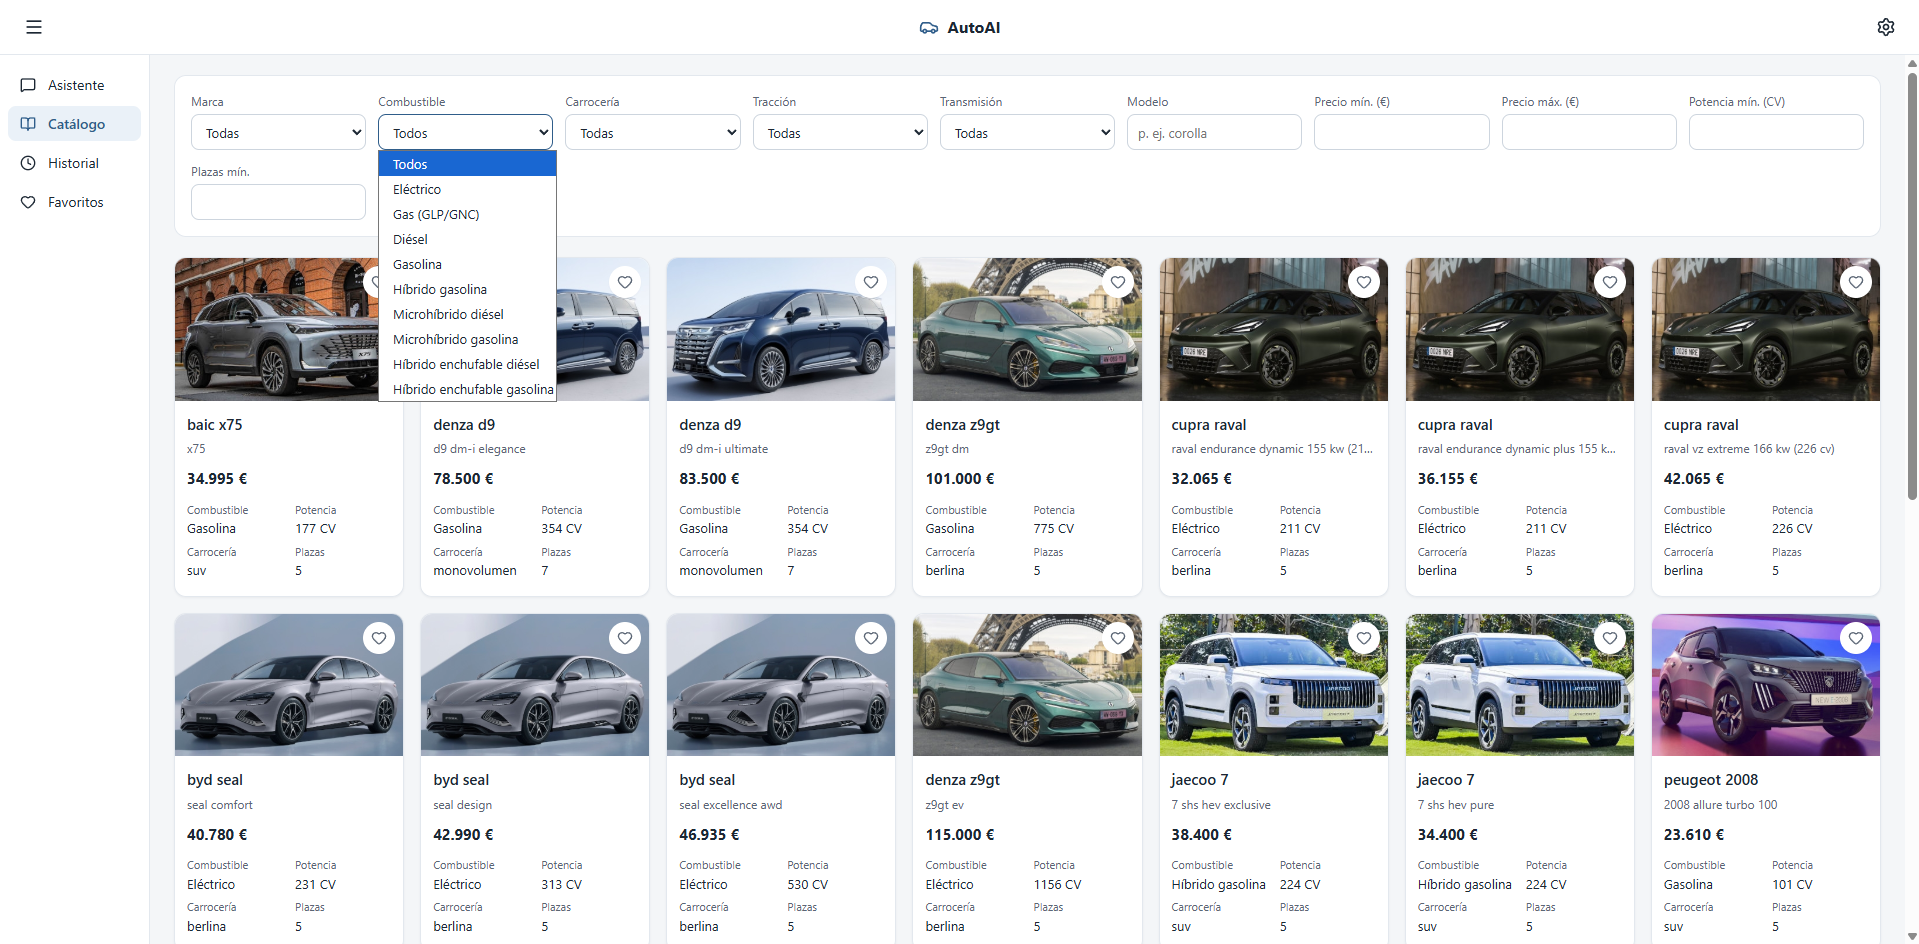
\includegraphics[width=1\textwidth]{Figuras/catalogo_filtros.png}
	\caption{Vista de catálogo con filtros.}
	\label{fig:catalogo-filtros}
\end{figure}


\subsubsection*{Favoritos e historial de consultas}

Por último, el diseño contempla dos funcionalidades de personalización
—\textbf{favoritos} e \textbf{historial}— con una decisión arquitectónica
deliberada: ambas se resuelven íntegramente en el lado del cliente, persistiendo
en el almacenamiento local del navegador, sin necesidad de cuentas de usuario ni
de almacenamiento en el servidor. Esta opción es coherente con el alcance del
proyecto —que no contempla la gestión de usuarios— y simplifica notablemente el
\emph{backend}, a costa de que la información quede ligada al navegador concreto.

Los favoritos permiten al usuario marcar vehículos de interés (desde las fichas
con imagen que genera el asistente o desde el catálogo) y revisarlos después en
una vista propia. El historial conserva las conversaciones mantenidas con el
asistente, agrupadas en sesiones con un título derivado de la primera pregunta,
de manera que el usuario pueda retomarlas o consultarlas más adelante. Para que
estas vistas se mantengan siempre sincronizadas con los cambios —incluso entre
varias pestañas abiertas simultáneamente—, la lectura del almacenamiento local se
integra con el sistema de reactividad de la interfaz, de modo que cualquier
modificación se refleja de inmediato en todas las vistas afectadas.

% Captura de pantalla de la vista de favoritos, mostrando
% una rejilla de tarjetas de vehículos marcados como favoritos, y de la vista de
% historial, mostrando una lista de conversaciones agrupadas en sesiones con su
% título derivado de la primera pregunta.

\begin{figure}[H]
    \centering
	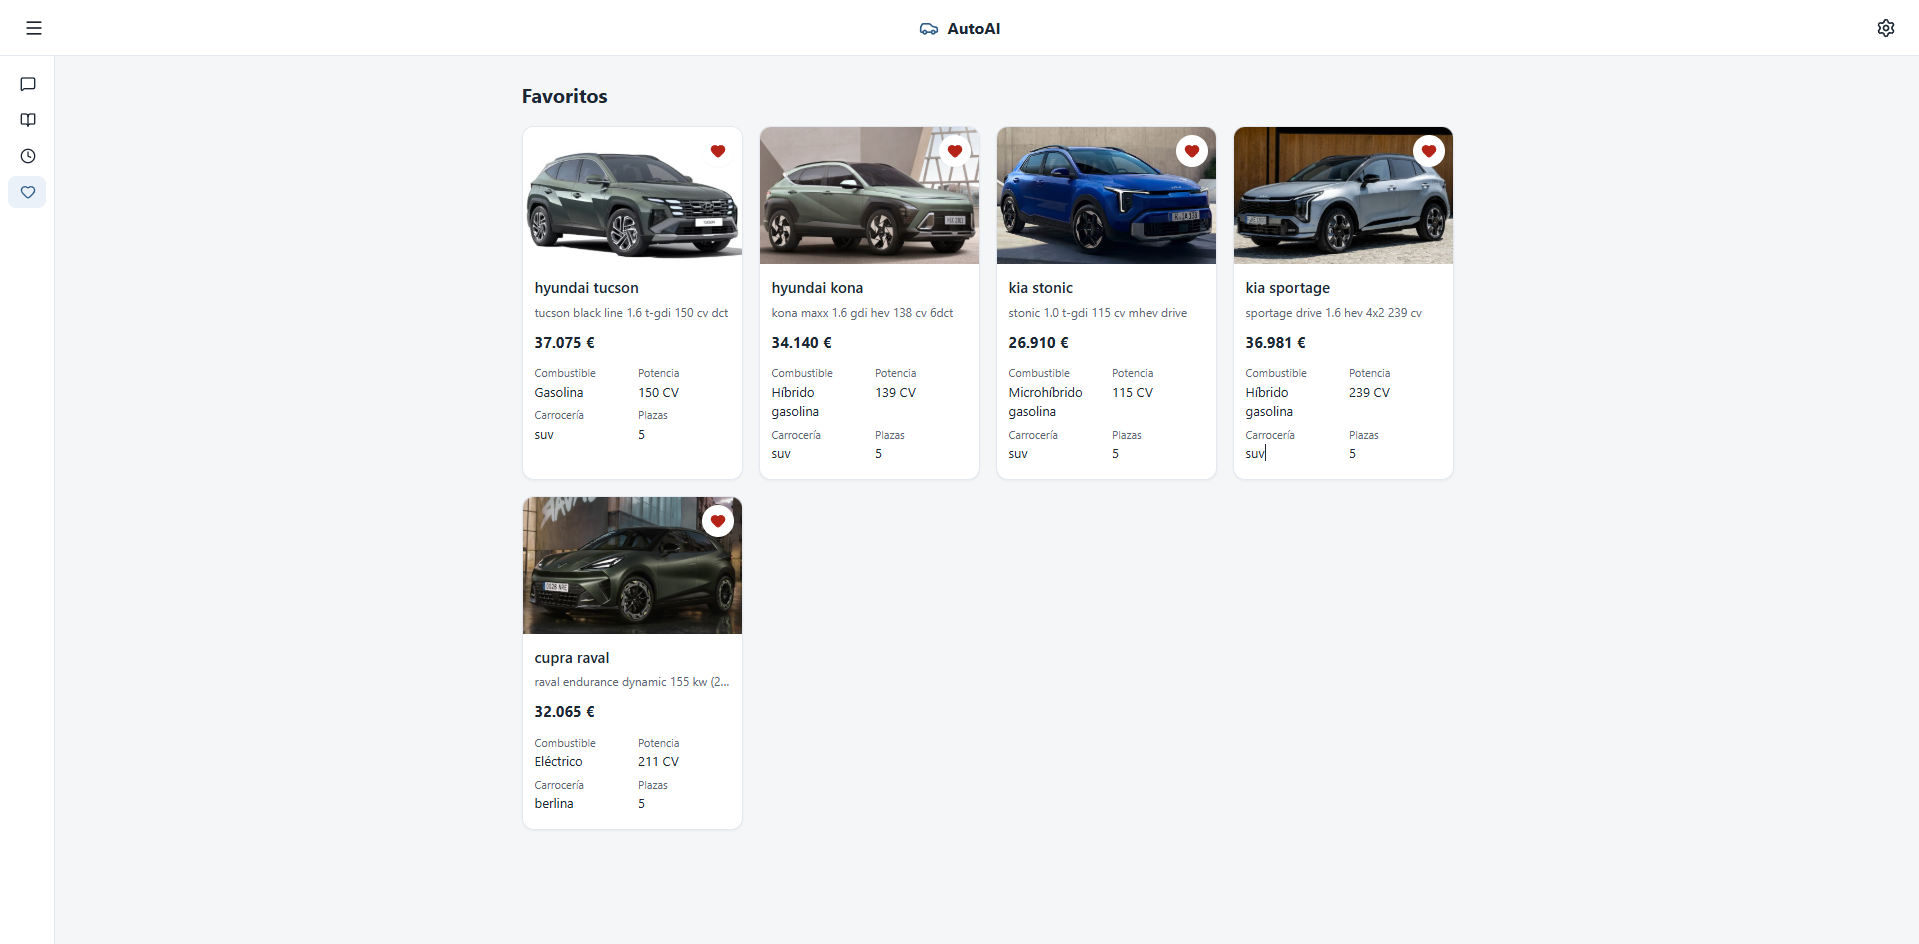
\includegraphics[width=1\textwidth]{Figuras/favoritos.png}
	\caption{Vista de favoritos.}
	\label{fig:favoritos}
\end{figure}

% Captura de pantalla de la vista de historial, mostrando una lista 
% de conversaciones agrupadas en sesiones con su título derivado de la primera
% pregunta, y de la vista de preferencias, mostrando opciones de tema claro/oscuro,
% tamaño de fuente e idioma de la interfaz.

\begin{figure}[H]
    \centering
	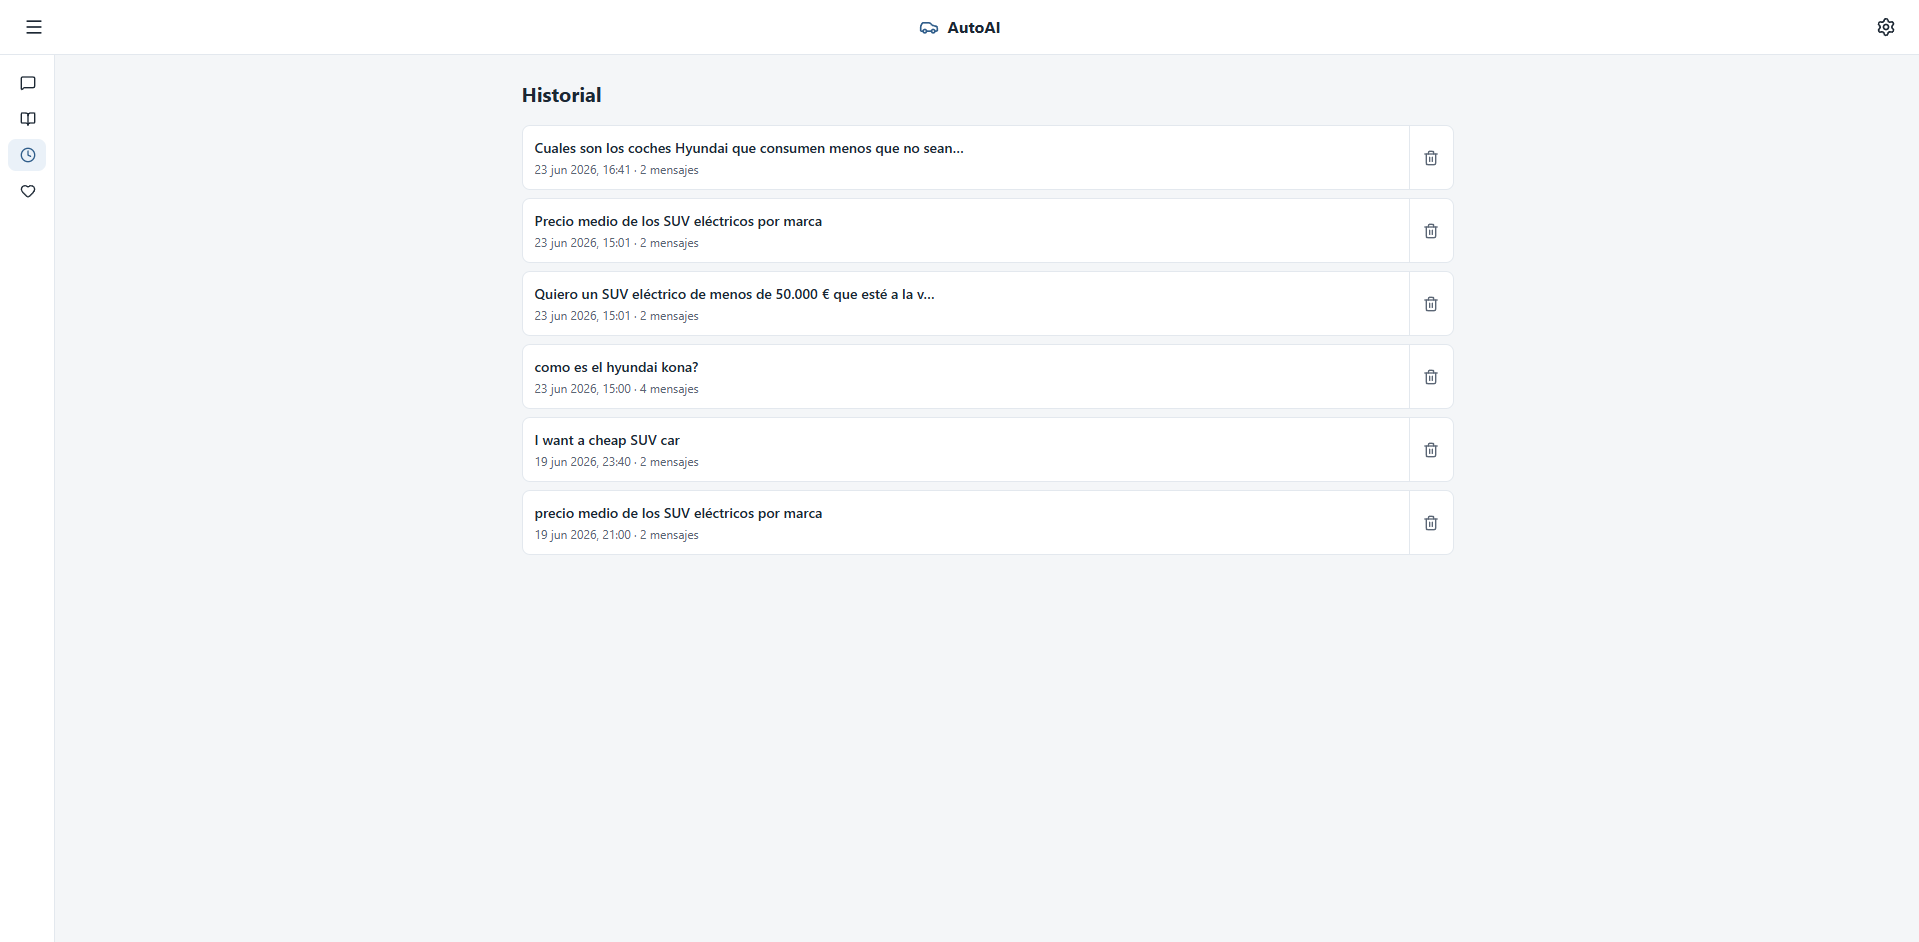
\includegraphics[width=1\textwidth]{Figuras/historial.png}
	\caption{Vista de historial.}
	\label{fig:historial}
\end{figure}

\subsubsection*{Preferencias de accesibilidad}

La interfaz incorpora un panel de \textbf{preferencias de accesibilidad} que
permite al usuario adaptar la presentación a sus necesidades. Se presenta como un
cajón lateral (\emph{drawer}) accesible —diseñado como diálogo modal con
atrapado del foco, cierre con la tecla \texttt{Esc} y navegación completa por
teclado— y reúne tres ajustes: el \textbf{tema} (claro u oscuro), el
\textbf{tamaño de la fuente} (reducido, normal o ampliado) y el \textbf{idioma}
de la interfaz (español o inglés). Coherentemente con la decisión adoptada para
favoritos e historial, estas preferencias también se resuelven en el lado del
cliente y persisten en el almacenamiento local del navegador, con unos valores
por defecto definidos (tema claro, tamaño normal e idioma español) y una lectura
defensiva que valida cada campo por separado y recurre al valor por defecto ante
cualquier dato corrupto.

El diseño de este panel persigue que cada ajuste tenga un efecto global e
inmediato sobre toda la aplicación, para lo cual cada preferencia se traduce en
un cambio sobre el documento raíz. El tema alterna un atributo en la raíz del
documento que conmuta la paleta de colores de toda la interfaz. El tamaño de
fuente, dado que toda la tipografía está expresada en unidades relativas, se
controla escalando un único valor en la raíz, lo que redimensiona la interfaz
\emph{proporcionalmente} sin romper la maquetación. El idioma, por su parte,
ajusta tanto el atributo de idioma del documento como el sistema de
internacionalización que traduce los textos de la interfaz; conviene recordar
aquí que la localización solo afecta a los textos propios de la aplicación y a la
prosa generada por el asistente, nunca a los datos de los vehículos.

Una última consideración de diseño atañe a la \textbf{experiencia de arranque}:
para evitar el destello visual que se produciría si la aplicación se cargara
primero con el tema por defecto y cambiara al tema preferido una vez iniciada,
las preferencias guardadas se aplican al documento \emph{antes} de que se monte
la interfaz. Así, el usuario percibe desde el primer instante la presentación que
había elegido.

% Captura de pantalla de la vista de preferencias, mostrando opciones de tema claro/oscuro,
% tamaño de fuente e idioma de la interfaz.

\begin{figure}[H]
    \centering
	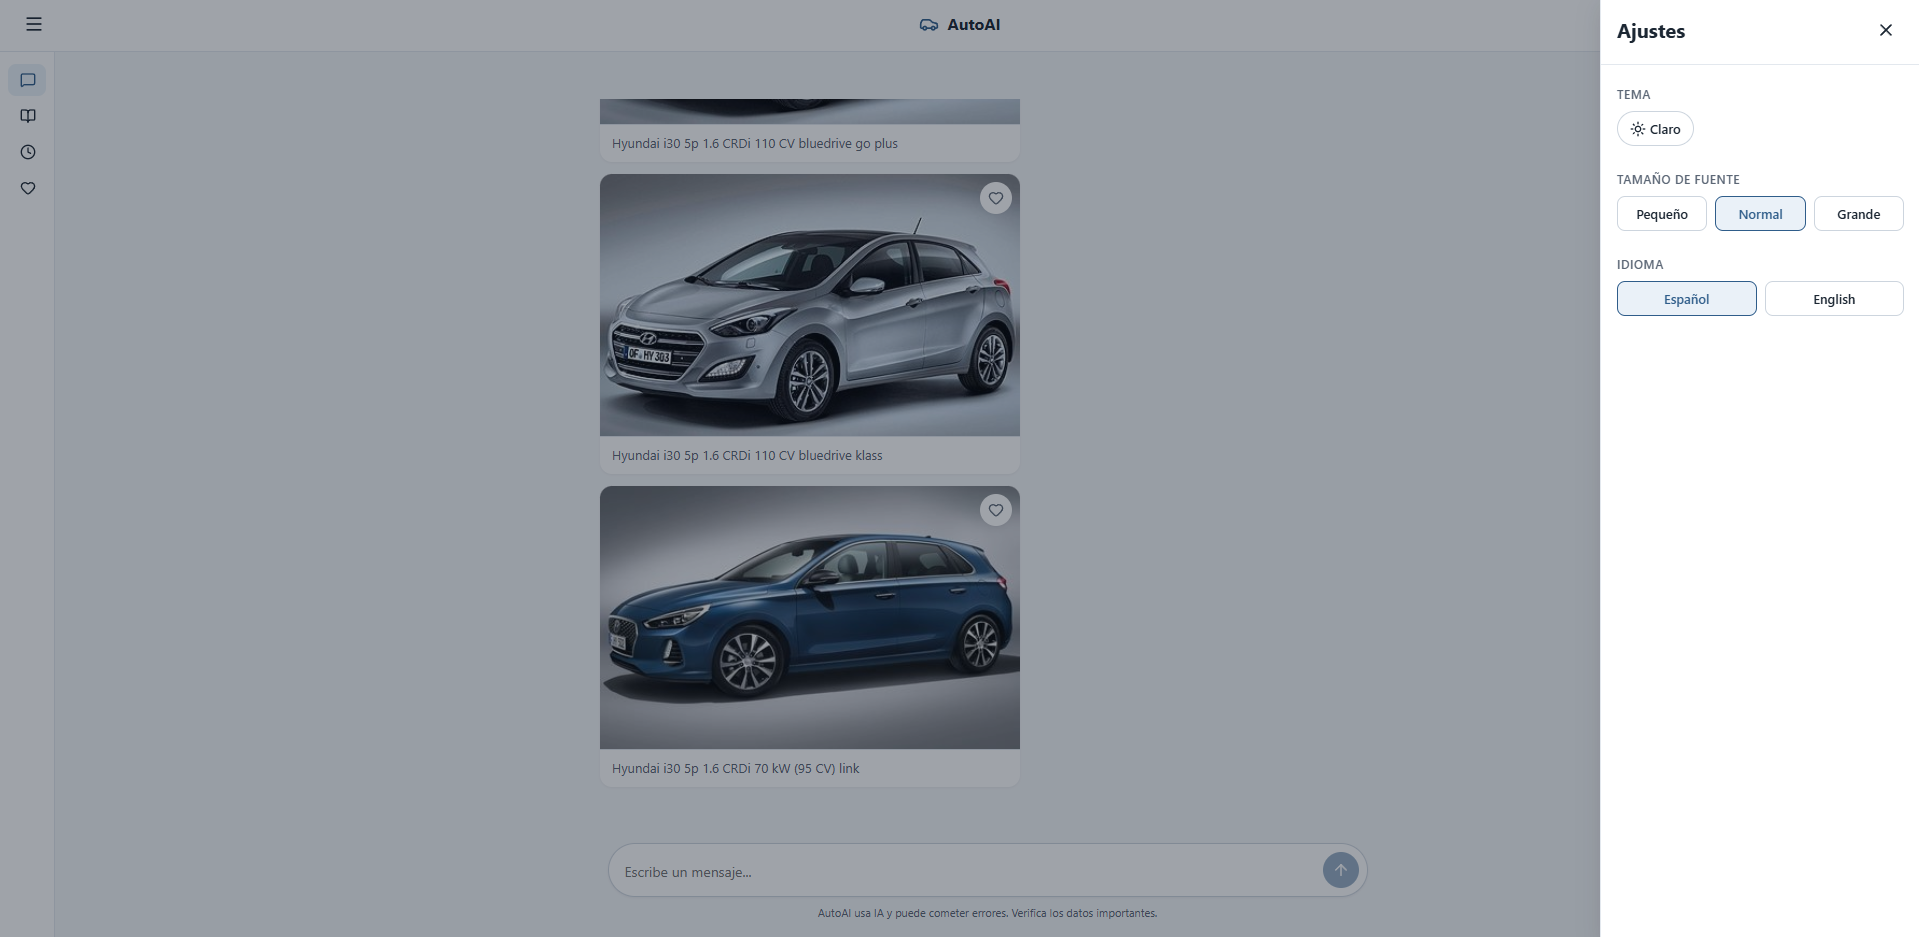
\includegraphics[width=1\textwidth]{Figuras/preferencias.png}
	\caption{Vista del panel de preferencias de accesibilidad.}
	\label{fig:preferencias}
\end{figure}


% ---------------------------------------------------------------------
%  6. IMPLEMENTACIÓN
% ---------------------------------------------------------------------
\chapter{Implementación}

\section{Obtención de datos: scraping de km77.com}

\subsection{Diseño del spider con Scrapy}

\subsection{Automatización periódica del scraping}

\section{Proceso ETL y carga en la base de datos}

\section{Backend con FastAPI}

\subsection{Endpoints del catálogo y comparador}

\subsection{Modelos de datos y validación}

\section{Integración de la inteligencia artificial}

\subsection{Traducción de lenguaje natural a filtros estructurados}

\subsection{Bucle de \textit{tool-calling} sobre datos reales}

\subsection{Generación de respuestas explicadas}

\section{Frontend con React}

\subsection{Interfaz conversacional}

\subsection{Catálogo, filtros y comparador}

\subsection{Favoritos e historial de consultas}

\section{Contenerización y despliegue con Docker}


% ---------------------------------------------------------------------
%  7. PRUEBAS Y EVALUACIÓN
% ---------------------------------------------------------------------
\chapter{Pruebas y evaluación}

\section{Estrategia de pruebas}

\section{Pruebas del backend y del pipeline de IA}

\section{Evaluación de la calidad de los resultados}

\section{Discusión de los resultados}


% ---------------------------------------------------------------------
%  8. CONCLUSIONES Y TRABAJO FUTURO
% ---------------------------------------------------------------------
\chapter{Conclusiones y trabajo futuro}

\section{Cumplimiento de los objetivos}

\section{Conclusiones}

\section{Líneas de trabajo futuro}
